\documentclass[border=5pt]{standalone}
\usepackage[T1]{fontenc}
\usepackage{lmodern,amsmath,amssymb,graphicx,tikz}
\usetikzlibrary{arrows.meta,calc}
\definecolor{ink}{HTML}{24302E}
\definecolor{muted}{HTML}{66716C}
\definecolor{linegray}{HTML}{D8DEDA}
\definecolor{gategray}{HTML}{F1F3F2}
\definecolor{green}{HTML}{326A4C}
\definecolor{palegreen}{HTML}{EDF4EE}
\newcommand{\head}[3]{\node[font=\fontsize{31}{34}\selectfont\bfseries] at (#1,473) {#3};}
\newcommand{\gate}[3]{\draw[fill=gategray,draw=ink,line width=1.2pt] (#1-21,#2-21) rectangle (#1+21,#2+21);\node[font=\fontsize{29}{32}\selectfont] at (#1,#2) {$#3$};}
\newcommand{\cx}[3]{\draw[ink,line width=1.5pt] (#1,#2)--(#1,#3);\fill[ink] (#1,#2) circle (4pt);\draw[fill=white,line width=1.5pt] (#1,#3) circle (8pt);\draw[line width=1.3pt] (#1-8,#3)--(#1+8,#3);\draw[line width=1.3pt] (#1,#3-8)--(#1,#3+8);}
\providecommand{\mathdefault}[1]{#1}
\begin{document}
\begin{tikzpicture}[x=1pt,y=1pt,text=ink,draw=ink,font=\fontsize{29}{33}\selectfont,>=Latex]
\path[use as bounding box] (0,0) rectangle (1520,500);
\head{190}{01}{Molecules}
\head{520}{02}{Coding agent}
\head{835}{03}{Circuit}
\head{1120}{04}{Certify}
\head{1405}{05}{Select}
% Larger data panel and type; identical frozen samples and binning.
\foreach \x/\name/\label in {52/CoH/CoH,144/O3/O_3,236/Na2/Na_2,328/NaLi/NaLi}{
 \node[font=\fontsize{28}{32}\selectfont] at (\x,430) {$\mathrm{\label}$};
 \node at (\x,392) {\includegraphics[width=75pt]{\name.png}};
}
\node at (190,203) {\resizebox{378pt}{!}{%% Creator: Matplotlib, PGF backend
%%
%% To include the figure in your LaTeX document, write
%%   \input{<filename>.pgf}
%%
%% Make sure the required packages are loaded in your preamble
%%   \usepackage{pgf}
%%
%% Also ensure that all the required font packages are loaded; for instance,
%% the lmodern package is sometimes necessary when using math font.
%%   \usepackage{lmodern}
%%
%% Figures using additional raster images can only be included by \input if
%% they are in the same directory as the main LaTeX file. For loading figures
%% from other directories you can use the `import` package
%%   \usepackage{import}
%%
%% and then include the figures with
%%   \import{<path to file>}{<filename>.pgf}
%%
%% Matplotlib used the following preamble
%%   \def\mathdefault#1{#1}
%%   \everymath=\expandafter{\the\everymath\displaystyle}
%%   \IfFileExists{scrextend.sty}{
%%     \usepackage[fontsize=27.000000pt]{scrextend}
%%   }{
%%     \renewcommand{\normalsize}{\fontsize{27.000000}{32.400000}\selectfont}
%%     \normalsize
%%   }
%%   \usepackage[T1]{fontenc}\usepackage{lmodern}\usepackage{amsmath}
%%   \makeatletter\@ifpackageloaded{underscore}{}{\usepackage[strings]{underscore}}\makeatother
%%
\begingroup%
\makeatletter%
\begin{pgfpicture}%
\pgfpathrectangle{\pgfpointorigin}{\pgfqpoint{5.250000in}{4.250000in}}%
\pgfusepath{use as bounding box, clip}%
\begin{pgfscope}%
\pgfsetbuttcap%
\pgfsetmiterjoin%
\definecolor{currentfill}{rgb}{1.000000,1.000000,1.000000}%
\pgfsetfillcolor{currentfill}%
\pgfsetlinewidth{0.000000pt}%
\definecolor{currentstroke}{rgb}{1.000000,1.000000,1.000000}%
\pgfsetstrokecolor{currentstroke}%
\pgfsetdash{}{0pt}%
\pgfpathmoveto{\pgfqpoint{0.000000in}{0.000000in}}%
\pgfpathlineto{\pgfqpoint{5.250000in}{0.000000in}}%
\pgfpathlineto{\pgfqpoint{5.250000in}{4.250000in}}%
\pgfpathlineto{\pgfqpoint{0.000000in}{4.250000in}}%
\pgfpathlineto{\pgfqpoint{0.000000in}{0.000000in}}%
\pgfpathclose%
\pgfusepath{fill}%
\end{pgfscope}%
\begin{pgfscope}%
\pgfsetbuttcap%
\pgfsetmiterjoin%
\definecolor{currentfill}{rgb}{1.000000,1.000000,1.000000}%
\pgfsetfillcolor{currentfill}%
\pgfsetlinewidth{0.000000pt}%
\definecolor{currentstroke}{rgb}{0.000000,0.000000,0.000000}%
\pgfsetstrokecolor{currentstroke}%
\pgfsetstrokeopacity{0.000000}%
\pgfsetdash{}{0pt}%
\pgfpathmoveto{\pgfqpoint{1.207500in}{2.584000in}}%
\pgfpathlineto{\pgfqpoint{3.009205in}{2.584000in}}%
\pgfpathlineto{\pgfqpoint{3.009205in}{3.740000in}}%
\pgfpathlineto{\pgfqpoint{1.207500in}{3.740000in}}%
\pgfpathlineto{\pgfqpoint{1.207500in}{2.584000in}}%
\pgfpathclose%
\pgfusepath{fill}%
\end{pgfscope}%
\begin{pgfscope}%
\pgfpathrectangle{\pgfqpoint{1.207500in}{2.584000in}}{\pgfqpoint{1.801705in}{1.156000in}}%
\pgfusepath{clip}%
\pgfsetbuttcap%
\pgfsetmiterjoin%
\definecolor{currentfill}{rgb}{0.462745,0.725490,0.000000}%
\pgfsetfillcolor{currentfill}%
\pgfsetfillopacity{0.350000}%
\pgfsetlinewidth{0.000000pt}%
\definecolor{currentstroke}{rgb}{0.000000,0.000000,0.000000}%
\pgfsetstrokecolor{currentstroke}%
\pgfsetstrokeopacity{0.350000}%
\pgfsetdash{}{0pt}%
\pgfpathmoveto{\pgfqpoint{1.289396in}{-226.701573in}}%
\pgfpathlineto{\pgfqpoint{1.289396in}{3.080515in}}%
\pgfpathlineto{\pgfqpoint{1.319727in}{3.080515in}}%
\pgfpathlineto{\pgfqpoint{1.319727in}{3.000790in}}%
\pgfpathlineto{\pgfqpoint{1.350059in}{3.000790in}}%
\pgfpathlineto{\pgfqpoint{1.350059in}{3.108920in}}%
\pgfpathlineto{\pgfqpoint{1.380391in}{3.108920in}}%
\pgfpathlineto{\pgfqpoint{1.380391in}{3.286972in}}%
\pgfpathlineto{\pgfqpoint{1.410723in}{3.286972in}}%
\pgfpathlineto{\pgfqpoint{1.410723in}{3.341819in}}%
\pgfpathlineto{\pgfqpoint{1.441054in}{3.341819in}}%
\pgfpathlineto{\pgfqpoint{1.441054in}{3.439354in}}%
\pgfpathlineto{\pgfqpoint{1.471386in}{3.439354in}}%
\pgfpathlineto{\pgfqpoint{1.471386in}{3.464977in}}%
\pgfpathlineto{\pgfqpoint{1.501718in}{3.464977in}}%
\pgfpathlineto{\pgfqpoint{1.501718in}{3.410576in}}%
\pgfpathlineto{\pgfqpoint{1.532049in}{3.410576in}}%
\pgfpathlineto{\pgfqpoint{1.532049in}{3.422256in}}%
\pgfpathlineto{\pgfqpoint{1.562381in}{3.422256in}}%
\pgfpathlineto{\pgfqpoint{1.562381in}{3.398463in}}%
\pgfpathlineto{\pgfqpoint{1.592713in}{3.398463in}}%
\pgfpathlineto{\pgfqpoint{1.592713in}{3.406173in}}%
\pgfpathlineto{\pgfqpoint{1.623045in}{3.406173in}}%
\pgfpathlineto{\pgfqpoint{1.623045in}{3.406173in}}%
\pgfpathlineto{\pgfqpoint{1.653376in}{3.406173in}}%
\pgfpathlineto{\pgfqpoint{1.653376in}{3.409853in}}%
\pgfpathlineto{\pgfqpoint{1.683708in}{3.409853in}}%
\pgfpathlineto{\pgfqpoint{1.683708in}{3.459298in}}%
\pgfpathlineto{\pgfqpoint{1.714040in}{3.459298in}}%
\pgfpathlineto{\pgfqpoint{1.714040in}{3.466356in}}%
\pgfpathlineto{\pgfqpoint{1.744372in}{3.466356in}}%
\pgfpathlineto{\pgfqpoint{1.744372in}{3.499766in}}%
\pgfpathlineto{\pgfqpoint{1.774703in}{3.499766in}}%
\pgfpathlineto{\pgfqpoint{1.774703in}{3.526832in}}%
\pgfpathlineto{\pgfqpoint{1.805035in}{3.526832in}}%
\pgfpathlineto{\pgfqpoint{1.805035in}{3.553785in}}%
\pgfpathlineto{\pgfqpoint{1.835367in}{3.553785in}}%
\pgfpathlineto{\pgfqpoint{1.835367in}{3.569924in}}%
\pgfpathlineto{\pgfqpoint{1.865698in}{3.569924in}}%
\pgfpathlineto{\pgfqpoint{1.865698in}{3.553336in}}%
\pgfpathlineto{\pgfqpoint{1.896030in}{3.553336in}}%
\pgfpathlineto{\pgfqpoint{1.896030in}{3.574738in}}%
\pgfpathlineto{\pgfqpoint{1.926362in}{3.574738in}}%
\pgfpathlineto{\pgfqpoint{1.926362in}{3.597583in}}%
\pgfpathlineto{\pgfqpoint{1.956694in}{3.597583in}}%
\pgfpathlineto{\pgfqpoint{1.956694in}{3.587119in}}%
\pgfpathlineto{\pgfqpoint{1.987025in}{3.587119in}}%
\pgfpathlineto{\pgfqpoint{1.987025in}{3.594568in}}%
\pgfpathlineto{\pgfqpoint{2.017357in}{3.594568in}}%
\pgfpathlineto{\pgfqpoint{2.017357in}{3.592626in}}%
\pgfpathlineto{\pgfqpoint{2.047689in}{3.592626in}}%
\pgfpathlineto{\pgfqpoint{2.047689in}{3.597269in}}%
\pgfpathlineto{\pgfqpoint{2.078021in}{3.597269in}}%
\pgfpathlineto{\pgfqpoint{2.078021in}{3.587800in}}%
\pgfpathlineto{\pgfqpoint{2.108352in}{3.587800in}}%
\pgfpathlineto{\pgfqpoint{2.108352in}{3.599757in}}%
\pgfpathlineto{\pgfqpoint{2.138684in}{3.599757in}}%
\pgfpathlineto{\pgfqpoint{2.138684in}{3.586435in}}%
\pgfpathlineto{\pgfqpoint{2.169016in}{3.586435in}}%
\pgfpathlineto{\pgfqpoint{2.169016in}{3.592463in}}%
\pgfpathlineto{\pgfqpoint{2.199347in}{3.592463in}}%
\pgfpathlineto{\pgfqpoint{2.199347in}{3.566741in}}%
\pgfpathlineto{\pgfqpoint{2.229679in}{3.566741in}}%
\pgfpathlineto{\pgfqpoint{2.229679in}{3.516043in}}%
\pgfpathlineto{\pgfqpoint{2.260011in}{3.516043in}}%
\pgfpathlineto{\pgfqpoint{2.260011in}{3.514200in}}%
\pgfpathlineto{\pgfqpoint{2.290343in}{3.514200in}}%
\pgfpathlineto{\pgfqpoint{2.290343in}{3.439354in}}%
\pgfpathlineto{\pgfqpoint{2.320674in}{3.439354in}}%
\pgfpathlineto{\pgfqpoint{2.320674in}{3.391926in}}%
\pgfpathlineto{\pgfqpoint{2.351006in}{3.391926in}}%
\pgfpathlineto{\pgfqpoint{2.351006in}{3.247701in}}%
\pgfpathlineto{\pgfqpoint{2.381338in}{3.247701in}}%
\pgfpathlineto{\pgfqpoint{2.381338in}{3.222883in}}%
\pgfpathlineto{\pgfqpoint{2.411670in}{3.222883in}}%
\pgfpathlineto{\pgfqpoint{2.411670in}{3.239974in}}%
\pgfpathlineto{\pgfqpoint{2.442001in}{3.239974in}}%
\pgfpathlineto{\pgfqpoint{2.442001in}{3.201040in}}%
\pgfpathlineto{\pgfqpoint{2.472333in}{3.201040in}}%
\pgfpathlineto{\pgfqpoint{2.472333in}{3.220356in}}%
\pgfpathlineto{\pgfqpoint{2.502665in}{3.220356in}}%
\pgfpathlineto{\pgfqpoint{2.502665in}{3.226982in}}%
\pgfpathlineto{\pgfqpoint{2.532996in}{3.226982in}}%
\pgfpathlineto{\pgfqpoint{2.532996in}{2.866164in}}%
\pgfpathlineto{\pgfqpoint{2.563328in}{2.866164in}}%
\pgfpathlineto{\pgfqpoint{2.563328in}{3.053834in}}%
\pgfpathlineto{\pgfqpoint{2.593660in}{3.053834in}}%
\pgfpathlineto{\pgfqpoint{2.593660in}{2.972163in}}%
\pgfpathlineto{\pgfqpoint{2.623992in}{2.972163in}}%
\pgfpathlineto{\pgfqpoint{2.623992in}{2.696284in}}%
\pgfpathlineto{\pgfqpoint{2.654323in}{2.696284in}}%
\pgfpathlineto{\pgfqpoint{2.654323in}{2.696284in}}%
\pgfpathlineto{\pgfqpoint{2.684655in}{2.696284in}}%
\pgfpathlineto{\pgfqpoint{2.684655in}{2.696284in}}%
\pgfpathlineto{\pgfqpoint{2.714987in}{2.696284in}}%
\pgfpathlineto{\pgfqpoint{2.714987in}{2.934740in}}%
\pgfpathlineto{\pgfqpoint{2.745319in}{2.934740in}}%
\pgfpathlineto{\pgfqpoint{2.745319in}{2.696284in}}%
\pgfpathlineto{\pgfqpoint{2.775650in}{2.696284in}}%
\pgfpathlineto{\pgfqpoint{2.775650in}{-226.701573in}}%
\pgfpathmoveto{\pgfqpoint{2.805982in}{-226.701573in}}%
\pgfpathlineto{\pgfqpoint{2.805982in}{2.830911in}}%
\pgfpathlineto{\pgfqpoint{2.836314in}{2.830911in}}%
\pgfpathlineto{\pgfqpoint{2.836314in}{2.696284in}}%
\pgfpathlineto{\pgfqpoint{2.866645in}{2.696284in}}%
\pgfpathlineto{\pgfqpoint{2.866645in}{-226.701573in}}%
\pgfusepath{fill}%
\end{pgfscope}%
\begin{pgfscope}%
\pgfsetbuttcap%
\pgfsetroundjoin%
\definecolor{currentfill}{rgb}{0.000000,0.000000,0.000000}%
\pgfsetfillcolor{currentfill}%
\pgfsetlinewidth{1.003750pt}%
\definecolor{currentstroke}{rgb}{0.000000,0.000000,0.000000}%
\pgfsetstrokecolor{currentstroke}%
\pgfsetdash{}{0pt}%
\pgfsys@defobject{currentmarker}{\pgfqpoint{0.000000in}{-0.055556in}}{\pgfqpoint{0.000000in}{0.000000in}}{%
\pgfpathmoveto{\pgfqpoint{0.000000in}{0.000000in}}%
\pgfpathlineto{\pgfqpoint{0.000000in}{-0.055556in}}%
\pgfusepath{stroke,fill}%
}%
\begin{pgfscope}%
\pgfsys@transformshift{1.616978in}{2.584000in}%
\pgfsys@useobject{currentmarker}{}%
\end{pgfscope}%
\end{pgfscope}%
\begin{pgfscope}%
\pgfsetbuttcap%
\pgfsetroundjoin%
\definecolor{currentfill}{rgb}{0.000000,0.000000,0.000000}%
\pgfsetfillcolor{currentfill}%
\pgfsetlinewidth{1.003750pt}%
\definecolor{currentstroke}{rgb}{0.000000,0.000000,0.000000}%
\pgfsetstrokecolor{currentstroke}%
\pgfsetdash{}{0pt}%
\pgfsys@defobject{currentmarker}{\pgfqpoint{0.000000in}{-0.055556in}}{\pgfqpoint{0.000000in}{0.000000in}}{%
\pgfpathmoveto{\pgfqpoint{0.000000in}{0.000000in}}%
\pgfpathlineto{\pgfqpoint{0.000000in}{-0.055556in}}%
\pgfusepath{stroke,fill}%
}%
\begin{pgfscope}%
\pgfsys@transformshift{2.435935in}{2.584000in}%
\pgfsys@useobject{currentmarker}{}%
\end{pgfscope}%
\end{pgfscope}%
\begin{pgfscope}%
\pgfsetbuttcap%
\pgfsetroundjoin%
\definecolor{currentfill}{rgb}{0.000000,0.000000,0.000000}%
\pgfsetfillcolor{currentfill}%
\pgfsetlinewidth{1.003750pt}%
\definecolor{currentstroke}{rgb}{0.000000,0.000000,0.000000}%
\pgfsetstrokecolor{currentstroke}%
\pgfsetdash{}{0pt}%
\pgfsys@defobject{currentmarker}{\pgfqpoint{-0.055556in}{0.000000in}}{\pgfqpoint{-0.000000in}{0.000000in}}{%
\pgfpathmoveto{\pgfqpoint{-0.000000in}{0.000000in}}%
\pgfpathlineto{\pgfqpoint{-0.055556in}{0.000000in}}%
\pgfusepath{stroke,fill}%
}%
\begin{pgfscope}%
\pgfsys@transformshift{1.207500in}{2.611345in}%
\pgfsys@useobject{currentmarker}{}%
\end{pgfscope}%
\end{pgfscope}%
\begin{pgfscope}%
\definecolor{textcolor}{rgb}{0.000000,0.000000,0.000000}%
\pgfsetstrokecolor{textcolor}%
\pgfsetfillcolor{textcolor}%
\pgftext[x=0.656177in, y=2.487986in, left, base]{\color{textcolor}{\rmfamily\fontsize{26.000000}{31.200000}\selectfont\catcode`\^=\active\def^{\ifmmode\sp\else\^{}\fi}\catcode`\%=\active\def%{\%}$\mathdefault{10^{0}}$}}%
\end{pgfscope}%
\begin{pgfscope}%
\pgfsetbuttcap%
\pgfsetroundjoin%
\definecolor{currentfill}{rgb}{0.000000,0.000000,0.000000}%
\pgfsetfillcolor{currentfill}%
\pgfsetlinewidth{1.003750pt}%
\definecolor{currentstroke}{rgb}{0.000000,0.000000,0.000000}%
\pgfsetstrokecolor{currentstroke}%
\pgfsetdash{}{0pt}%
\pgfsys@defobject{currentmarker}{\pgfqpoint{-0.055556in}{0.000000in}}{\pgfqpoint{-0.000000in}{0.000000in}}{%
\pgfpathmoveto{\pgfqpoint{-0.000000in}{0.000000in}}%
\pgfpathlineto{\pgfqpoint{-0.055556in}{0.000000in}}%
\pgfusepath{stroke,fill}%
}%
\begin{pgfscope}%
\pgfsys@transformshift{1.207500in}{3.175672in}%
\pgfsys@useobject{currentmarker}{}%
\end{pgfscope}%
\end{pgfscope}%
\begin{pgfscope}%
\definecolor{textcolor}{rgb}{0.000000,0.000000,0.000000}%
\pgfsetstrokecolor{textcolor}%
\pgfsetfillcolor{textcolor}%
\pgftext[x=0.656177in, y=3.052314in, left, base]{\color{textcolor}{\rmfamily\fontsize{26.000000}{31.200000}\selectfont\catcode`\^=\active\def^{\ifmmode\sp\else\^{}\fi}\catcode`\%=\active\def%{\%}$\mathdefault{10^{2}}$}}%
\end{pgfscope}%
\begin{pgfscope}%
\pgfsetbuttcap%
\pgfsetroundjoin%
\definecolor{currentfill}{rgb}{0.000000,0.000000,0.000000}%
\pgfsetfillcolor{currentfill}%
\pgfsetlinewidth{1.003750pt}%
\definecolor{currentstroke}{rgb}{0.000000,0.000000,0.000000}%
\pgfsetstrokecolor{currentstroke}%
\pgfsetdash{}{0pt}%
\pgfsys@defobject{currentmarker}{\pgfqpoint{-0.055556in}{0.000000in}}{\pgfqpoint{-0.000000in}{0.000000in}}{%
\pgfpathmoveto{\pgfqpoint{-0.000000in}{0.000000in}}%
\pgfpathlineto{\pgfqpoint{-0.055556in}{0.000000in}}%
\pgfusepath{stroke,fill}%
}%
\begin{pgfscope}%
\pgfsys@transformshift{1.207500in}{3.740000in}%
\pgfsys@useobject{currentmarker}{}%
\end{pgfscope}%
\end{pgfscope}%
\begin{pgfscope}%
\definecolor{textcolor}{rgb}{0.000000,0.000000,0.000000}%
\pgfsetstrokecolor{textcolor}%
\pgfsetfillcolor{textcolor}%
\pgftext[x=0.656177in, y=3.616641in, left, base]{\color{textcolor}{\rmfamily\fontsize{26.000000}{31.200000}\selectfont\catcode`\^=\active\def^{\ifmmode\sp\else\^{}\fi}\catcode`\%=\active\def%{\%}$\mathdefault{10^{4}}$}}%
\end{pgfscope}%
\begin{pgfscope}%
\pgfpathrectangle{\pgfqpoint{1.207500in}{2.584000in}}{\pgfqpoint{1.801705in}{1.156000in}}%
\pgfusepath{clip}%
\pgfsetbuttcap%
\pgfsetmiterjoin%
\pgfsetlinewidth{1.104125pt}%
\definecolor{currentstroke}{rgb}{0.243137,0.494118,0.000000}%
\pgfsetstrokecolor{currentstroke}%
\pgfsetdash{}{0pt}%
\pgfpathmoveto{\pgfqpoint{1.289396in}{2.574000in}}%
\pgfpathlineto{\pgfqpoint{1.289396in}{3.080515in}}%
\pgfpathlineto{\pgfqpoint{1.319727in}{3.080515in}}%
\pgfpathlineto{\pgfqpoint{1.319727in}{3.000790in}}%
\pgfpathlineto{\pgfqpoint{1.350059in}{3.000790in}}%
\pgfpathlineto{\pgfqpoint{1.350059in}{3.108920in}}%
\pgfpathlineto{\pgfqpoint{1.380391in}{3.108920in}}%
\pgfpathlineto{\pgfqpoint{1.380391in}{3.286972in}}%
\pgfpathlineto{\pgfqpoint{1.410723in}{3.286972in}}%
\pgfpathlineto{\pgfqpoint{1.410723in}{3.341819in}}%
\pgfpathlineto{\pgfqpoint{1.441054in}{3.341819in}}%
\pgfpathlineto{\pgfqpoint{1.441054in}{3.439354in}}%
\pgfpathlineto{\pgfqpoint{1.471386in}{3.439354in}}%
\pgfpathlineto{\pgfqpoint{1.471386in}{3.464977in}}%
\pgfpathlineto{\pgfqpoint{1.501718in}{3.464977in}}%
\pgfpathlineto{\pgfqpoint{1.501718in}{3.410576in}}%
\pgfpathlineto{\pgfqpoint{1.532049in}{3.410576in}}%
\pgfpathlineto{\pgfqpoint{1.532049in}{3.422256in}}%
\pgfpathlineto{\pgfqpoint{1.562381in}{3.422256in}}%
\pgfpathlineto{\pgfqpoint{1.562381in}{3.398463in}}%
\pgfpathlineto{\pgfqpoint{1.592713in}{3.398463in}}%
\pgfpathlineto{\pgfqpoint{1.592713in}{3.406173in}}%
\pgfpathlineto{\pgfqpoint{1.623045in}{3.406173in}}%
\pgfpathlineto{\pgfqpoint{1.623045in}{3.406173in}}%
\pgfpathlineto{\pgfqpoint{1.653376in}{3.406173in}}%
\pgfpathlineto{\pgfqpoint{1.653376in}{3.409853in}}%
\pgfpathlineto{\pgfqpoint{1.683708in}{3.409853in}}%
\pgfpathlineto{\pgfqpoint{1.683708in}{3.459298in}}%
\pgfpathlineto{\pgfqpoint{1.714040in}{3.459298in}}%
\pgfpathlineto{\pgfqpoint{1.714040in}{3.466356in}}%
\pgfpathlineto{\pgfqpoint{1.744372in}{3.466356in}}%
\pgfpathlineto{\pgfqpoint{1.744372in}{3.499766in}}%
\pgfpathlineto{\pgfqpoint{1.774703in}{3.499766in}}%
\pgfpathlineto{\pgfqpoint{1.774703in}{3.526832in}}%
\pgfpathlineto{\pgfqpoint{1.805035in}{3.526832in}}%
\pgfpathlineto{\pgfqpoint{1.805035in}{3.553785in}}%
\pgfpathlineto{\pgfqpoint{1.835367in}{3.553785in}}%
\pgfpathlineto{\pgfqpoint{1.835367in}{3.569924in}}%
\pgfpathlineto{\pgfqpoint{1.865698in}{3.569924in}}%
\pgfpathlineto{\pgfqpoint{1.865698in}{3.553336in}}%
\pgfpathlineto{\pgfqpoint{1.896030in}{3.553336in}}%
\pgfpathlineto{\pgfqpoint{1.896030in}{3.574738in}}%
\pgfpathlineto{\pgfqpoint{1.926362in}{3.574738in}}%
\pgfpathlineto{\pgfqpoint{1.926362in}{3.597583in}}%
\pgfpathlineto{\pgfqpoint{1.956694in}{3.597583in}}%
\pgfpathlineto{\pgfqpoint{1.956694in}{3.587119in}}%
\pgfpathlineto{\pgfqpoint{1.987025in}{3.587119in}}%
\pgfpathlineto{\pgfqpoint{1.987025in}{3.594568in}}%
\pgfpathlineto{\pgfqpoint{2.017357in}{3.594568in}}%
\pgfpathlineto{\pgfqpoint{2.017357in}{3.592626in}}%
\pgfpathlineto{\pgfqpoint{2.047689in}{3.592626in}}%
\pgfpathlineto{\pgfqpoint{2.047689in}{3.597269in}}%
\pgfpathlineto{\pgfqpoint{2.078021in}{3.597269in}}%
\pgfpathlineto{\pgfqpoint{2.078021in}{3.587800in}}%
\pgfpathlineto{\pgfqpoint{2.108352in}{3.587800in}}%
\pgfpathlineto{\pgfqpoint{2.108352in}{3.599757in}}%
\pgfpathlineto{\pgfqpoint{2.138684in}{3.599757in}}%
\pgfpathlineto{\pgfqpoint{2.138684in}{3.586435in}}%
\pgfpathlineto{\pgfqpoint{2.169016in}{3.586435in}}%
\pgfpathlineto{\pgfqpoint{2.169016in}{3.592463in}}%
\pgfpathlineto{\pgfqpoint{2.199347in}{3.592463in}}%
\pgfpathlineto{\pgfqpoint{2.199347in}{3.566741in}}%
\pgfpathlineto{\pgfqpoint{2.229679in}{3.566741in}}%
\pgfpathlineto{\pgfqpoint{2.229679in}{3.516043in}}%
\pgfpathlineto{\pgfqpoint{2.260011in}{3.516043in}}%
\pgfpathlineto{\pgfqpoint{2.260011in}{3.514200in}}%
\pgfpathlineto{\pgfqpoint{2.290343in}{3.514200in}}%
\pgfpathlineto{\pgfqpoint{2.290343in}{3.439354in}}%
\pgfpathlineto{\pgfqpoint{2.320674in}{3.439354in}}%
\pgfpathlineto{\pgfqpoint{2.320674in}{3.391926in}}%
\pgfpathlineto{\pgfqpoint{2.351006in}{3.391926in}}%
\pgfpathlineto{\pgfqpoint{2.351006in}{3.247701in}}%
\pgfpathlineto{\pgfqpoint{2.381338in}{3.247701in}}%
\pgfpathlineto{\pgfqpoint{2.381338in}{3.222883in}}%
\pgfpathlineto{\pgfqpoint{2.411670in}{3.222883in}}%
\pgfpathlineto{\pgfqpoint{2.411670in}{3.239974in}}%
\pgfpathlineto{\pgfqpoint{2.442001in}{3.239974in}}%
\pgfpathlineto{\pgfqpoint{2.442001in}{3.201040in}}%
\pgfpathlineto{\pgfqpoint{2.472333in}{3.201040in}}%
\pgfpathlineto{\pgfqpoint{2.472333in}{3.220356in}}%
\pgfpathlineto{\pgfqpoint{2.502665in}{3.220356in}}%
\pgfpathlineto{\pgfqpoint{2.502665in}{3.226982in}}%
\pgfpathlineto{\pgfqpoint{2.532996in}{3.226982in}}%
\pgfpathlineto{\pgfqpoint{2.532996in}{2.866164in}}%
\pgfpathlineto{\pgfqpoint{2.563328in}{2.866164in}}%
\pgfpathlineto{\pgfqpoint{2.563328in}{3.053834in}}%
\pgfpathlineto{\pgfqpoint{2.593660in}{3.053834in}}%
\pgfpathlineto{\pgfqpoint{2.593660in}{2.972163in}}%
\pgfpathlineto{\pgfqpoint{2.623992in}{2.972163in}}%
\pgfpathlineto{\pgfqpoint{2.623992in}{2.696284in}}%
\pgfpathlineto{\pgfqpoint{2.654323in}{2.696284in}}%
\pgfpathlineto{\pgfqpoint{2.654323in}{2.696284in}}%
\pgfpathlineto{\pgfqpoint{2.684655in}{2.696284in}}%
\pgfpathlineto{\pgfqpoint{2.684655in}{2.696284in}}%
\pgfpathlineto{\pgfqpoint{2.714987in}{2.696284in}}%
\pgfpathlineto{\pgfqpoint{2.714987in}{2.934740in}}%
\pgfpathlineto{\pgfqpoint{2.745319in}{2.934740in}}%
\pgfpathlineto{\pgfqpoint{2.745319in}{2.696284in}}%
\pgfpathlineto{\pgfqpoint{2.775650in}{2.696284in}}%
\pgfpathlineto{\pgfqpoint{2.775650in}{2.574000in}}%
\pgfpathmoveto{\pgfqpoint{2.805982in}{2.574000in}}%
\pgfpathlineto{\pgfqpoint{2.805982in}{2.830911in}}%
\pgfpathlineto{\pgfqpoint{2.836314in}{2.830911in}}%
\pgfpathlineto{\pgfqpoint{2.836314in}{2.696284in}}%
\pgfpathlineto{\pgfqpoint{2.866645in}{2.696284in}}%
\pgfpathlineto{\pgfqpoint{2.866645in}{2.574000in}}%
\pgfusepath{stroke}%
\end{pgfscope}%
\begin{pgfscope}%
\pgfsetrectcap%
\pgfsetmiterjoin%
\pgfsetlinewidth{1.003750pt}%
\definecolor{currentstroke}{rgb}{0.000000,0.000000,0.000000}%
\pgfsetstrokecolor{currentstroke}%
\pgfsetdash{}{0pt}%
\pgfpathmoveto{\pgfqpoint{1.207500in}{2.584000in}}%
\pgfpathlineto{\pgfqpoint{1.207500in}{3.740000in}}%
\pgfusepath{stroke}%
\end{pgfscope}%
\begin{pgfscope}%
\pgfsetrectcap%
\pgfsetmiterjoin%
\pgfsetlinewidth{1.003750pt}%
\definecolor{currentstroke}{rgb}{0.000000,0.000000,0.000000}%
\pgfsetstrokecolor{currentstroke}%
\pgfsetdash{}{0pt}%
\pgfpathmoveto{\pgfqpoint{3.009205in}{2.584000in}}%
\pgfpathlineto{\pgfqpoint{3.009205in}{3.740000in}}%
\pgfusepath{stroke}%
\end{pgfscope}%
\begin{pgfscope}%
\pgfsetrectcap%
\pgfsetmiterjoin%
\pgfsetlinewidth{1.003750pt}%
\definecolor{currentstroke}{rgb}{0.000000,0.000000,0.000000}%
\pgfsetstrokecolor{currentstroke}%
\pgfsetdash{}{0pt}%
\pgfpathmoveto{\pgfqpoint{1.207500in}{2.584000in}}%
\pgfpathlineto{\pgfqpoint{3.009205in}{2.584000in}}%
\pgfusepath{stroke}%
\end{pgfscope}%
\begin{pgfscope}%
\pgfsetrectcap%
\pgfsetmiterjoin%
\pgfsetlinewidth{1.003750pt}%
\definecolor{currentstroke}{rgb}{0.000000,0.000000,0.000000}%
\pgfsetstrokecolor{currentstroke}%
\pgfsetdash{}{0pt}%
\pgfpathmoveto{\pgfqpoint{1.207500in}{3.740000in}}%
\pgfpathlineto{\pgfqpoint{3.009205in}{3.740000in}}%
\pgfusepath{stroke}%
\end{pgfscope}%
\begin{pgfscope}%
\definecolor{textcolor}{rgb}{0.000000,0.000000,0.000000}%
\pgfsetstrokecolor{textcolor}%
\pgfsetfillcolor{textcolor}%
\pgftext[x=2.108352in,y=3.837222in,,base]{\color{textcolor}{\rmfamily\fontsize{26.000000}{31.200000}\selectfont\catcode`\^=\active\def^{\ifmmode\sp\else\^{}\fi}\catcode`\%=\active\def%{\%}$\mathrm{CoH}$ (30 Q)}}%
\end{pgfscope}%
\begin{pgfscope}%
\pgfsetbuttcap%
\pgfsetmiterjoin%
\definecolor{currentfill}{rgb}{1.000000,1.000000,1.000000}%
\pgfsetfillcolor{currentfill}%
\pgfsetlinewidth{0.000000pt}%
\definecolor{currentstroke}{rgb}{0.000000,0.000000,0.000000}%
\pgfsetstrokecolor{currentstroke}%
\pgfsetstrokeopacity{0.000000}%
\pgfsetdash{}{0pt}%
\pgfpathmoveto{\pgfqpoint{3.369545in}{2.584000in}}%
\pgfpathlineto{\pgfqpoint{5.171250in}{2.584000in}}%
\pgfpathlineto{\pgfqpoint{5.171250in}{3.740000in}}%
\pgfpathlineto{\pgfqpoint{3.369545in}{3.740000in}}%
\pgfpathlineto{\pgfqpoint{3.369545in}{2.584000in}}%
\pgfpathclose%
\pgfusepath{fill}%
\end{pgfscope}%
\begin{pgfscope}%
\pgfpathrectangle{\pgfqpoint{3.369545in}{2.584000in}}{\pgfqpoint{1.801705in}{1.156000in}}%
\pgfusepath{clip}%
\pgfsetbuttcap%
\pgfsetmiterjoin%
\definecolor{currentfill}{rgb}{0.462745,0.725490,0.000000}%
\pgfsetfillcolor{currentfill}%
\pgfsetfillopacity{0.350000}%
\pgfsetlinewidth{0.000000pt}%
\definecolor{currentstroke}{rgb}{0.000000,0.000000,0.000000}%
\pgfsetstrokecolor{currentstroke}%
\pgfsetstrokeopacity{0.350000}%
\pgfsetdash{}{0pt}%
\pgfpathmoveto{\pgfqpoint{3.694095in}{-226.701573in}}%
\pgfpathlineto{\pgfqpoint{3.694095in}{2.866164in}}%
\pgfpathlineto{\pgfqpoint{3.724427in}{2.866164in}}%
\pgfpathlineto{\pgfqpoint{3.724427in}{-226.701573in}}%
\pgfpathmoveto{\pgfqpoint{3.906417in}{-226.701573in}}%
\pgfpathlineto{\pgfqpoint{3.906417in}{2.951104in}}%
\pgfpathlineto{\pgfqpoint{3.936749in}{2.951104in}}%
\pgfpathlineto{\pgfqpoint{3.936749in}{2.866164in}}%
\pgfpathlineto{\pgfqpoint{3.967080in}{2.866164in}}%
\pgfpathlineto{\pgfqpoint{3.967080in}{2.781224in}}%
\pgfpathlineto{\pgfqpoint{3.997412in}{2.781224in}}%
\pgfpathlineto{\pgfqpoint{3.997412in}{2.978448in}}%
\pgfpathlineto{\pgfqpoint{4.027744in}{2.978448in}}%
\pgfpathlineto{\pgfqpoint{4.027744in}{2.866164in}}%
\pgfpathlineto{\pgfqpoint{4.058076in}{2.866164in}}%
\pgfpathlineto{\pgfqpoint{4.058076in}{3.000790in}}%
\pgfpathlineto{\pgfqpoint{4.088407in}{3.000790in}}%
\pgfpathlineto{\pgfqpoint{4.088407in}{2.978448in}}%
\pgfpathlineto{\pgfqpoint{4.118739in}{2.978448in}}%
\pgfpathlineto{\pgfqpoint{4.118739in}{3.050477in}}%
\pgfpathlineto{\pgfqpoint{4.149071in}{3.050477in}}%
\pgfpathlineto{\pgfqpoint{4.149071in}{3.189560in}}%
\pgfpathlineto{\pgfqpoint{4.179403in}{3.189560in}}%
\pgfpathlineto{\pgfqpoint{4.179403in}{3.193860in}}%
\pgfpathlineto{\pgfqpoint{4.209734in}{3.193860in}}%
\pgfpathlineto{\pgfqpoint{4.209734in}{3.284980in}}%
\pgfpathlineto{\pgfqpoint{4.240066in}{3.284980in}}%
\pgfpathlineto{\pgfqpoint{4.240066in}{3.216904in}}%
\pgfpathlineto{\pgfqpoint{4.270398in}{3.216904in}}%
\pgfpathlineto{\pgfqpoint{4.270398in}{3.315105in}}%
\pgfpathlineto{\pgfqpoint{4.300729in}{3.315105in}}%
\pgfpathlineto{\pgfqpoint{4.300729in}{3.361608in}}%
\pgfpathlineto{\pgfqpoint{4.331061in}{3.361608in}}%
\pgfpathlineto{\pgfqpoint{4.331061in}{3.385905in}}%
\pgfpathlineto{\pgfqpoint{4.361393in}{3.385905in}}%
\pgfpathlineto{\pgfqpoint{4.361393in}{3.409853in}}%
\pgfpathlineto{\pgfqpoint{4.391725in}{3.409853in}}%
\pgfpathlineto{\pgfqpoint{4.391725in}{3.415521in}}%
\pgfpathlineto{\pgfqpoint{4.422056in}{3.415521in}}%
\pgfpathlineto{\pgfqpoint{4.422056in}{3.418935in}}%
\pgfpathlineto{\pgfqpoint{4.452388in}{3.418935in}}%
\pgfpathlineto{\pgfqpoint{4.452388in}{3.391084in}}%
\pgfpathlineto{\pgfqpoint{4.482720in}{3.391084in}}%
\pgfpathlineto{\pgfqpoint{4.482720in}{3.328486in}}%
\pgfpathlineto{\pgfqpoint{4.513052in}{3.328486in}}%
\pgfpathlineto{\pgfqpoint{4.513052in}{3.120983in}}%
\pgfpathlineto{\pgfqpoint{4.543383in}{3.120983in}}%
\pgfpathlineto{\pgfqpoint{4.543383in}{2.781224in}}%
\pgfpathlineto{\pgfqpoint{4.573715in}{2.781224in}}%
\pgfpathlineto{\pgfqpoint{4.573715in}{3.175672in}}%
\pgfpathlineto{\pgfqpoint{4.604047in}{3.175672in}}%
\pgfpathlineto{\pgfqpoint{4.604047in}{3.229377in}}%
\pgfpathlineto{\pgfqpoint{4.634378in}{3.229377in}}%
\pgfpathlineto{\pgfqpoint{4.634378in}{-226.701573in}}%
\pgfpathmoveto{\pgfqpoint{4.786037in}{-226.701573in}}%
\pgfpathlineto{\pgfqpoint{4.786037in}{2.965537in}}%
\pgfpathlineto{\pgfqpoint{4.816369in}{2.965537in}}%
\pgfpathlineto{\pgfqpoint{4.816369in}{2.781224in}}%
\pgfpathlineto{\pgfqpoint{4.846701in}{2.781224in}}%
\pgfpathlineto{\pgfqpoint{4.846701in}{-226.701573in}}%
\pgfusepath{fill}%
\end{pgfscope}%
\begin{pgfscope}%
\pgfsetbuttcap%
\pgfsetroundjoin%
\definecolor{currentfill}{rgb}{0.000000,0.000000,0.000000}%
\pgfsetfillcolor{currentfill}%
\pgfsetlinewidth{1.003750pt}%
\definecolor{currentstroke}{rgb}{0.000000,0.000000,0.000000}%
\pgfsetstrokecolor{currentstroke}%
\pgfsetdash{}{0pt}%
\pgfsys@defobject{currentmarker}{\pgfqpoint{0.000000in}{-0.055556in}}{\pgfqpoint{0.000000in}{0.000000in}}{%
\pgfpathmoveto{\pgfqpoint{0.000000in}{0.000000in}}%
\pgfpathlineto{\pgfqpoint{0.000000in}{-0.055556in}}%
\pgfusepath{stroke,fill}%
}%
\begin{pgfscope}%
\pgfsys@transformshift{3.779024in}{2.584000in}%
\pgfsys@useobject{currentmarker}{}%
\end{pgfscope}%
\end{pgfscope}%
\begin{pgfscope}%
\pgfsetbuttcap%
\pgfsetroundjoin%
\definecolor{currentfill}{rgb}{0.000000,0.000000,0.000000}%
\pgfsetfillcolor{currentfill}%
\pgfsetlinewidth{1.003750pt}%
\definecolor{currentstroke}{rgb}{0.000000,0.000000,0.000000}%
\pgfsetstrokecolor{currentstroke}%
\pgfsetdash{}{0pt}%
\pgfsys@defobject{currentmarker}{\pgfqpoint{0.000000in}{-0.055556in}}{\pgfqpoint{0.000000in}{0.000000in}}{%
\pgfpathmoveto{\pgfqpoint{0.000000in}{0.000000in}}%
\pgfpathlineto{\pgfqpoint{0.000000in}{-0.055556in}}%
\pgfusepath{stroke,fill}%
}%
\begin{pgfscope}%
\pgfsys@transformshift{4.597980in}{2.584000in}%
\pgfsys@useobject{currentmarker}{}%
\end{pgfscope}%
\end{pgfscope}%
\begin{pgfscope}%
\pgfsetbuttcap%
\pgfsetroundjoin%
\definecolor{currentfill}{rgb}{0.000000,0.000000,0.000000}%
\pgfsetfillcolor{currentfill}%
\pgfsetlinewidth{1.003750pt}%
\definecolor{currentstroke}{rgb}{0.000000,0.000000,0.000000}%
\pgfsetstrokecolor{currentstroke}%
\pgfsetdash{}{0pt}%
\pgfsys@defobject{currentmarker}{\pgfqpoint{-0.055556in}{0.000000in}}{\pgfqpoint{-0.000000in}{0.000000in}}{%
\pgfpathmoveto{\pgfqpoint{-0.000000in}{0.000000in}}%
\pgfpathlineto{\pgfqpoint{-0.055556in}{0.000000in}}%
\pgfusepath{stroke,fill}%
}%
\begin{pgfscope}%
\pgfsys@transformshift{3.369545in}{2.611345in}%
\pgfsys@useobject{currentmarker}{}%
\end{pgfscope}%
\end{pgfscope}%
\begin{pgfscope}%
\pgfsetbuttcap%
\pgfsetroundjoin%
\definecolor{currentfill}{rgb}{0.000000,0.000000,0.000000}%
\pgfsetfillcolor{currentfill}%
\pgfsetlinewidth{1.003750pt}%
\definecolor{currentstroke}{rgb}{0.000000,0.000000,0.000000}%
\pgfsetstrokecolor{currentstroke}%
\pgfsetdash{}{0pt}%
\pgfsys@defobject{currentmarker}{\pgfqpoint{-0.055556in}{0.000000in}}{\pgfqpoint{-0.000000in}{0.000000in}}{%
\pgfpathmoveto{\pgfqpoint{-0.000000in}{0.000000in}}%
\pgfpathlineto{\pgfqpoint{-0.055556in}{0.000000in}}%
\pgfusepath{stroke,fill}%
}%
\begin{pgfscope}%
\pgfsys@transformshift{3.369545in}{3.175672in}%
\pgfsys@useobject{currentmarker}{}%
\end{pgfscope}%
\end{pgfscope}%
\begin{pgfscope}%
\pgfsetbuttcap%
\pgfsetroundjoin%
\definecolor{currentfill}{rgb}{0.000000,0.000000,0.000000}%
\pgfsetfillcolor{currentfill}%
\pgfsetlinewidth{1.003750pt}%
\definecolor{currentstroke}{rgb}{0.000000,0.000000,0.000000}%
\pgfsetstrokecolor{currentstroke}%
\pgfsetdash{}{0pt}%
\pgfsys@defobject{currentmarker}{\pgfqpoint{-0.055556in}{0.000000in}}{\pgfqpoint{-0.000000in}{0.000000in}}{%
\pgfpathmoveto{\pgfqpoint{-0.000000in}{0.000000in}}%
\pgfpathlineto{\pgfqpoint{-0.055556in}{0.000000in}}%
\pgfusepath{stroke,fill}%
}%
\begin{pgfscope}%
\pgfsys@transformshift{3.369545in}{3.740000in}%
\pgfsys@useobject{currentmarker}{}%
\end{pgfscope}%
\end{pgfscope}%
\begin{pgfscope}%
\pgfpathrectangle{\pgfqpoint{3.369545in}{2.584000in}}{\pgfqpoint{1.801705in}{1.156000in}}%
\pgfusepath{clip}%
\pgfsetbuttcap%
\pgfsetmiterjoin%
\pgfsetlinewidth{1.104125pt}%
\definecolor{currentstroke}{rgb}{0.243137,0.494118,0.000000}%
\pgfsetstrokecolor{currentstroke}%
\pgfsetdash{}{0pt}%
\pgfpathmoveto{\pgfqpoint{3.694095in}{2.574000in}}%
\pgfpathlineto{\pgfqpoint{3.694095in}{2.866164in}}%
\pgfpathlineto{\pgfqpoint{3.724427in}{2.866164in}}%
\pgfpathlineto{\pgfqpoint{3.724427in}{2.574000in}}%
\pgfpathmoveto{\pgfqpoint{3.906417in}{2.574000in}}%
\pgfpathlineto{\pgfqpoint{3.906417in}{2.951104in}}%
\pgfpathlineto{\pgfqpoint{3.936749in}{2.951104in}}%
\pgfpathlineto{\pgfqpoint{3.936749in}{2.866164in}}%
\pgfpathlineto{\pgfqpoint{3.967080in}{2.866164in}}%
\pgfpathlineto{\pgfqpoint{3.967080in}{2.781224in}}%
\pgfpathlineto{\pgfqpoint{3.997412in}{2.781224in}}%
\pgfpathlineto{\pgfqpoint{3.997412in}{2.978448in}}%
\pgfpathlineto{\pgfqpoint{4.027744in}{2.978448in}}%
\pgfpathlineto{\pgfqpoint{4.027744in}{2.866164in}}%
\pgfpathlineto{\pgfqpoint{4.058076in}{2.866164in}}%
\pgfpathlineto{\pgfqpoint{4.058076in}{3.000790in}}%
\pgfpathlineto{\pgfqpoint{4.088407in}{3.000790in}}%
\pgfpathlineto{\pgfqpoint{4.088407in}{2.978448in}}%
\pgfpathlineto{\pgfqpoint{4.118739in}{2.978448in}}%
\pgfpathlineto{\pgfqpoint{4.118739in}{3.050477in}}%
\pgfpathlineto{\pgfqpoint{4.149071in}{3.050477in}}%
\pgfpathlineto{\pgfqpoint{4.149071in}{3.189560in}}%
\pgfpathlineto{\pgfqpoint{4.179403in}{3.189560in}}%
\pgfpathlineto{\pgfqpoint{4.179403in}{3.193860in}}%
\pgfpathlineto{\pgfqpoint{4.209734in}{3.193860in}}%
\pgfpathlineto{\pgfqpoint{4.209734in}{3.284980in}}%
\pgfpathlineto{\pgfqpoint{4.240066in}{3.284980in}}%
\pgfpathlineto{\pgfqpoint{4.240066in}{3.216904in}}%
\pgfpathlineto{\pgfqpoint{4.270398in}{3.216904in}}%
\pgfpathlineto{\pgfqpoint{4.270398in}{3.315105in}}%
\pgfpathlineto{\pgfqpoint{4.300729in}{3.315105in}}%
\pgfpathlineto{\pgfqpoint{4.300729in}{3.361608in}}%
\pgfpathlineto{\pgfqpoint{4.331061in}{3.361608in}}%
\pgfpathlineto{\pgfqpoint{4.331061in}{3.385905in}}%
\pgfpathlineto{\pgfqpoint{4.361393in}{3.385905in}}%
\pgfpathlineto{\pgfqpoint{4.361393in}{3.409853in}}%
\pgfpathlineto{\pgfqpoint{4.391725in}{3.409853in}}%
\pgfpathlineto{\pgfqpoint{4.391725in}{3.415521in}}%
\pgfpathlineto{\pgfqpoint{4.422056in}{3.415521in}}%
\pgfpathlineto{\pgfqpoint{4.422056in}{3.418935in}}%
\pgfpathlineto{\pgfqpoint{4.452388in}{3.418935in}}%
\pgfpathlineto{\pgfqpoint{4.452388in}{3.391084in}}%
\pgfpathlineto{\pgfqpoint{4.482720in}{3.391084in}}%
\pgfpathlineto{\pgfqpoint{4.482720in}{3.328486in}}%
\pgfpathlineto{\pgfqpoint{4.513052in}{3.328486in}}%
\pgfpathlineto{\pgfqpoint{4.513052in}{3.120983in}}%
\pgfpathlineto{\pgfqpoint{4.543383in}{3.120983in}}%
\pgfpathlineto{\pgfqpoint{4.543383in}{2.781224in}}%
\pgfpathlineto{\pgfqpoint{4.573715in}{2.781224in}}%
\pgfpathlineto{\pgfqpoint{4.573715in}{3.175672in}}%
\pgfpathlineto{\pgfqpoint{4.604047in}{3.175672in}}%
\pgfpathlineto{\pgfqpoint{4.604047in}{3.229377in}}%
\pgfpathlineto{\pgfqpoint{4.634378in}{3.229377in}}%
\pgfpathlineto{\pgfqpoint{4.634378in}{2.574000in}}%
\pgfpathmoveto{\pgfqpoint{4.786037in}{2.574000in}}%
\pgfpathlineto{\pgfqpoint{4.786037in}{2.965537in}}%
\pgfpathlineto{\pgfqpoint{4.816369in}{2.965537in}}%
\pgfpathlineto{\pgfqpoint{4.816369in}{2.781224in}}%
\pgfpathlineto{\pgfqpoint{4.846701in}{2.781224in}}%
\pgfpathlineto{\pgfqpoint{4.846701in}{2.574000in}}%
\pgfusepath{stroke}%
\end{pgfscope}%
\begin{pgfscope}%
\pgfsetrectcap%
\pgfsetmiterjoin%
\pgfsetlinewidth{1.003750pt}%
\definecolor{currentstroke}{rgb}{0.000000,0.000000,0.000000}%
\pgfsetstrokecolor{currentstroke}%
\pgfsetdash{}{0pt}%
\pgfpathmoveto{\pgfqpoint{3.369545in}{2.584000in}}%
\pgfpathlineto{\pgfqpoint{3.369545in}{3.740000in}}%
\pgfusepath{stroke}%
\end{pgfscope}%
\begin{pgfscope}%
\pgfsetrectcap%
\pgfsetmiterjoin%
\pgfsetlinewidth{1.003750pt}%
\definecolor{currentstroke}{rgb}{0.000000,0.000000,0.000000}%
\pgfsetstrokecolor{currentstroke}%
\pgfsetdash{}{0pt}%
\pgfpathmoveto{\pgfqpoint{5.171250in}{2.584000in}}%
\pgfpathlineto{\pgfqpoint{5.171250in}{3.740000in}}%
\pgfusepath{stroke}%
\end{pgfscope}%
\begin{pgfscope}%
\pgfsetrectcap%
\pgfsetmiterjoin%
\pgfsetlinewidth{1.003750pt}%
\definecolor{currentstroke}{rgb}{0.000000,0.000000,0.000000}%
\pgfsetstrokecolor{currentstroke}%
\pgfsetdash{}{0pt}%
\pgfpathmoveto{\pgfqpoint{3.369545in}{2.584000in}}%
\pgfpathlineto{\pgfqpoint{5.171250in}{2.584000in}}%
\pgfusepath{stroke}%
\end{pgfscope}%
\begin{pgfscope}%
\pgfsetrectcap%
\pgfsetmiterjoin%
\pgfsetlinewidth{1.003750pt}%
\definecolor{currentstroke}{rgb}{0.000000,0.000000,0.000000}%
\pgfsetstrokecolor{currentstroke}%
\pgfsetdash{}{0pt}%
\pgfpathmoveto{\pgfqpoint{3.369545in}{3.740000in}}%
\pgfpathlineto{\pgfqpoint{5.171250in}{3.740000in}}%
\pgfusepath{stroke}%
\end{pgfscope}%
\begin{pgfscope}%
\definecolor{textcolor}{rgb}{0.000000,0.000000,0.000000}%
\pgfsetstrokecolor{textcolor}%
\pgfsetfillcolor{textcolor}%
\pgftext[x=4.270398in,y=3.837222in,,base]{\color{textcolor}{\rmfamily\fontsize{26.000000}{31.200000}\selectfont\catcode`\^=\active\def^{\ifmmode\sp\else\^{}\fi}\catcode`\%=\active\def%{\%}$\mathrm{O}_3$ (22 Q)}}%
\end{pgfscope}%
\begin{pgfscope}%
\pgfsetbuttcap%
\pgfsetmiterjoin%
\definecolor{currentfill}{rgb}{1.000000,1.000000,1.000000}%
\pgfsetfillcolor{currentfill}%
\pgfsetlinewidth{0.000000pt}%
\definecolor{currentstroke}{rgb}{0.000000,0.000000,0.000000}%
\pgfsetstrokecolor{currentstroke}%
\pgfsetstrokeopacity{0.000000}%
\pgfsetdash{}{0pt}%
\pgfpathmoveto{\pgfqpoint{1.207500in}{0.850000in}}%
\pgfpathlineto{\pgfqpoint{3.009205in}{0.850000in}}%
\pgfpathlineto{\pgfqpoint{3.009205in}{2.006000in}}%
\pgfpathlineto{\pgfqpoint{1.207500in}{2.006000in}}%
\pgfpathlineto{\pgfqpoint{1.207500in}{0.850000in}}%
\pgfpathclose%
\pgfusepath{fill}%
\end{pgfscope}%
\begin{pgfscope}%
\pgfpathrectangle{\pgfqpoint{1.207500in}{0.850000in}}{\pgfqpoint{1.801705in}{1.156000in}}%
\pgfusepath{clip}%
\pgfsetbuttcap%
\pgfsetmiterjoin%
\definecolor{currentfill}{rgb}{0.462745,0.725490,0.000000}%
\pgfsetfillcolor{currentfill}%
\pgfsetfillopacity{0.350000}%
\pgfsetlinewidth{0.000000pt}%
\definecolor{currentstroke}{rgb}{0.000000,0.000000,0.000000}%
\pgfsetstrokecolor{currentstroke}%
\pgfsetstrokeopacity{0.350000}%
\pgfsetdash{}{0pt}%
\pgfpathmoveto{\pgfqpoint{1.441054in}{-226.701573in}}%
\pgfpathlineto{\pgfqpoint{1.441054in}{1.132164in}}%
\pgfpathlineto{\pgfqpoint{1.471386in}{1.132164in}}%
\pgfpathlineto{\pgfqpoint{1.471386in}{-226.701573in}}%
\pgfpathmoveto{\pgfqpoint{1.501718in}{-226.701573in}}%
\pgfpathlineto{\pgfqpoint{1.501718in}{1.244448in}}%
\pgfpathlineto{\pgfqpoint{1.532049in}{1.244448in}}%
\pgfpathlineto{\pgfqpoint{1.532049in}{1.132164in}}%
\pgfpathlineto{\pgfqpoint{1.562381in}{1.132164in}}%
\pgfpathlineto{\pgfqpoint{1.562381in}{1.132164in}}%
\pgfpathlineto{\pgfqpoint{1.592713in}{1.132164in}}%
\pgfpathlineto{\pgfqpoint{1.592713in}{1.217104in}}%
\pgfpathlineto{\pgfqpoint{1.623045in}{1.217104in}}%
\pgfpathlineto{\pgfqpoint{1.623045in}{-226.701573in}}%
\pgfpathmoveto{\pgfqpoint{1.653376in}{-226.701573in}}%
\pgfpathlineto{\pgfqpoint{1.653376in}{1.329388in}}%
\pgfpathlineto{\pgfqpoint{1.683708in}{1.329388in}}%
\pgfpathlineto{\pgfqpoint{1.683708in}{1.302043in}}%
\pgfpathlineto{\pgfqpoint{1.714040in}{1.302043in}}%
\pgfpathlineto{\pgfqpoint{1.714040in}{1.446478in}}%
\pgfpathlineto{\pgfqpoint{1.744372in}{1.446478in}}%
\pgfpathlineto{\pgfqpoint{1.744372in}{1.132164in}}%
\pgfpathlineto{\pgfqpoint{1.774703in}{1.132164in}}%
\pgfpathlineto{\pgfqpoint{1.774703in}{1.244448in}}%
\pgfpathlineto{\pgfqpoint{1.805035in}{1.244448in}}%
\pgfpathlineto{\pgfqpoint{1.805035in}{1.341067in}}%
\pgfpathlineto{\pgfqpoint{1.835367in}{1.341067in}}%
\pgfpathlineto{\pgfqpoint{1.835367in}{1.379075in}}%
\pgfpathlineto{\pgfqpoint{1.865698in}{1.379075in}}%
\pgfpathlineto{\pgfqpoint{1.865698in}{1.431454in}}%
\pgfpathlineto{\pgfqpoint{1.896030in}{1.431454in}}%
\pgfpathlineto{\pgfqpoint{1.896030in}{1.420307in}}%
\pgfpathlineto{\pgfqpoint{1.926362in}{1.420307in}}%
\pgfpathlineto{\pgfqpoint{1.926362in}{1.431454in}}%
\pgfpathlineto{\pgfqpoint{1.956694in}{1.431454in}}%
\pgfpathlineto{\pgfqpoint{1.956694in}{1.529039in}}%
\pgfpathlineto{\pgfqpoint{1.987025in}{1.529039in}}%
\pgfpathlineto{\pgfqpoint{1.987025in}{1.556863in}}%
\pgfpathlineto{\pgfqpoint{2.017357in}{1.556863in}}%
\pgfpathlineto{\pgfqpoint{2.017357in}{1.302043in}}%
\pgfpathlineto{\pgfqpoint{2.047689in}{1.302043in}}%
\pgfpathlineto{\pgfqpoint{2.047689in}{1.446478in}}%
\pgfpathlineto{\pgfqpoint{2.078021in}{1.446478in}}%
\pgfpathlineto{\pgfqpoint{2.078021in}{1.436670in}}%
\pgfpathlineto{\pgfqpoint{2.108352in}{1.436670in}}%
\pgfpathlineto{\pgfqpoint{2.108352in}{1.526612in}}%
\pgfpathlineto{\pgfqpoint{2.138684in}{1.526612in}}%
\pgfpathlineto{\pgfqpoint{2.138684in}{1.590186in}}%
\pgfpathlineto{\pgfqpoint{2.169016in}{1.590186in}}%
\pgfpathlineto{\pgfqpoint{2.169016in}{1.526612in}}%
\pgfpathlineto{\pgfqpoint{2.199347in}{1.526612in}}%
\pgfpathlineto{\pgfqpoint{2.199347in}{1.505246in}}%
\pgfpathlineto{\pgfqpoint{2.229679in}{1.505246in}}%
\pgfpathlineto{\pgfqpoint{2.229679in}{1.489714in}}%
\pgfpathlineto{\pgfqpoint{2.260011in}{1.489714in}}%
\pgfpathlineto{\pgfqpoint{2.260011in}{1.471923in}}%
\pgfpathlineto{\pgfqpoint{2.290343in}{1.471923in}}%
\pgfpathlineto{\pgfqpoint{2.290343in}{-226.701573in}}%
\pgfpathmoveto{\pgfqpoint{2.320674in}{-226.701573in}}%
\pgfpathlineto{\pgfqpoint{2.320674in}{1.439197in}}%
\pgfpathlineto{\pgfqpoint{2.351006in}{1.439197in}}%
\pgfpathlineto{\pgfqpoint{2.351006in}{1.368412in}}%
\pgfpathlineto{\pgfqpoint{2.381338in}{1.368412in}}%
\pgfpathlineto{\pgfqpoint{2.381338in}{1.332414in}}%
\pgfpathlineto{\pgfqpoint{2.411670in}{1.332414in}}%
\pgfpathlineto{\pgfqpoint{2.411670in}{1.266790in}}%
\pgfpathlineto{\pgfqpoint{2.442001in}{1.266790in}}%
\pgfpathlineto{\pgfqpoint{2.442001in}{1.519030in}}%
\pgfpathlineto{\pgfqpoint{2.472333in}{1.519030in}}%
\pgfpathlineto{\pgfqpoint{2.472333in}{1.217104in}}%
\pgfpathlineto{\pgfqpoint{2.502665in}{1.217104in}}%
\pgfpathlineto{\pgfqpoint{2.502665in}{-226.701573in}}%
\pgfpathmoveto{\pgfqpoint{2.563328in}{-226.701573in}}%
\pgfpathlineto{\pgfqpoint{2.563328in}{0.962284in}}%
\pgfpathlineto{\pgfqpoint{2.593660in}{0.962284in}}%
\pgfpathlineto{\pgfqpoint{2.593660in}{0.962284in}}%
\pgfpathlineto{\pgfqpoint{2.623992in}{0.962284in}}%
\pgfpathlineto{\pgfqpoint{2.623992in}{-226.701573in}}%
\pgfpathmoveto{\pgfqpoint{2.654323in}{-226.701573in}}%
\pgfpathlineto{\pgfqpoint{2.654323in}{1.181850in}}%
\pgfpathlineto{\pgfqpoint{2.684655in}{1.181850in}}%
\pgfpathlineto{\pgfqpoint{2.684655in}{1.047224in}}%
\pgfpathlineto{\pgfqpoint{2.714987in}{1.047224in}}%
\pgfpathlineto{\pgfqpoint{2.714987in}{-226.701573in}}%
\pgfusepath{fill}%
\end{pgfscope}%
\begin{pgfscope}%
\pgfsetbuttcap%
\pgfsetroundjoin%
\definecolor{currentfill}{rgb}{0.000000,0.000000,0.000000}%
\pgfsetfillcolor{currentfill}%
\pgfsetlinewidth{1.003750pt}%
\definecolor{currentstroke}{rgb}{0.000000,0.000000,0.000000}%
\pgfsetstrokecolor{currentstroke}%
\pgfsetdash{}{0pt}%
\pgfsys@defobject{currentmarker}{\pgfqpoint{0.000000in}{-0.055556in}}{\pgfqpoint{0.000000in}{0.000000in}}{%
\pgfpathmoveto{\pgfqpoint{0.000000in}{0.000000in}}%
\pgfpathlineto{\pgfqpoint{0.000000in}{-0.055556in}}%
\pgfusepath{stroke,fill}%
}%
\begin{pgfscope}%
\pgfsys@transformshift{1.616978in}{0.850000in}%
\pgfsys@useobject{currentmarker}{}%
\end{pgfscope}%
\end{pgfscope}%
\begin{pgfscope}%
\definecolor{textcolor}{rgb}{0.000000,0.000000,0.000000}%
\pgfsetstrokecolor{textcolor}%
\pgfsetfillcolor{textcolor}%
\pgftext[x=1.616978in,y=0.752778in,,top]{\color{textcolor}{\rmfamily\fontsize{24.000000}{28.800000}\selectfont\catcode`\^=\active\def^{\ifmmode\sp\else\^{}\fi}\catcode`\%=\active\def%{\%}$\mathdefault{10^{-6}}$}}%
\end{pgfscope}%
\begin{pgfscope}%
\pgfsetbuttcap%
\pgfsetroundjoin%
\definecolor{currentfill}{rgb}{0.000000,0.000000,0.000000}%
\pgfsetfillcolor{currentfill}%
\pgfsetlinewidth{1.003750pt}%
\definecolor{currentstroke}{rgb}{0.000000,0.000000,0.000000}%
\pgfsetstrokecolor{currentstroke}%
\pgfsetdash{}{0pt}%
\pgfsys@defobject{currentmarker}{\pgfqpoint{0.000000in}{-0.055556in}}{\pgfqpoint{0.000000in}{0.000000in}}{%
\pgfpathmoveto{\pgfqpoint{0.000000in}{0.000000in}}%
\pgfpathlineto{\pgfqpoint{0.000000in}{-0.055556in}}%
\pgfusepath{stroke,fill}%
}%
\begin{pgfscope}%
\pgfsys@transformshift{2.435935in}{0.850000in}%
\pgfsys@useobject{currentmarker}{}%
\end{pgfscope}%
\end{pgfscope}%
\begin{pgfscope}%
\definecolor{textcolor}{rgb}{0.000000,0.000000,0.000000}%
\pgfsetstrokecolor{textcolor}%
\pgfsetfillcolor{textcolor}%
\pgftext[x=2.435935in,y=0.752778in,,top]{\color{textcolor}{\rmfamily\fontsize{24.000000}{28.800000}\selectfont\catcode`\^=\active\def^{\ifmmode\sp\else\^{}\fi}\catcode`\%=\active\def%{\%}$\mathdefault{10^{-1}}$}}%
\end{pgfscope}%
\begin{pgfscope}%
\pgfsetbuttcap%
\pgfsetroundjoin%
\definecolor{currentfill}{rgb}{0.000000,0.000000,0.000000}%
\pgfsetfillcolor{currentfill}%
\pgfsetlinewidth{1.003750pt}%
\definecolor{currentstroke}{rgb}{0.000000,0.000000,0.000000}%
\pgfsetstrokecolor{currentstroke}%
\pgfsetdash{}{0pt}%
\pgfsys@defobject{currentmarker}{\pgfqpoint{-0.055556in}{0.000000in}}{\pgfqpoint{-0.000000in}{0.000000in}}{%
\pgfpathmoveto{\pgfqpoint{-0.000000in}{0.000000in}}%
\pgfpathlineto{\pgfqpoint{-0.055556in}{0.000000in}}%
\pgfusepath{stroke,fill}%
}%
\begin{pgfscope}%
\pgfsys@transformshift{1.207500in}{0.877345in}%
\pgfsys@useobject{currentmarker}{}%
\end{pgfscope}%
\end{pgfscope}%
\begin{pgfscope}%
\definecolor{textcolor}{rgb}{0.000000,0.000000,0.000000}%
\pgfsetstrokecolor{textcolor}%
\pgfsetfillcolor{textcolor}%
\pgftext[x=0.656177in, y=0.753986in, left, base]{\color{textcolor}{\rmfamily\fontsize{26.000000}{31.200000}\selectfont\catcode`\^=\active\def^{\ifmmode\sp\else\^{}\fi}\catcode`\%=\active\def%{\%}$\mathdefault{10^{0}}$}}%
\end{pgfscope}%
\begin{pgfscope}%
\pgfsetbuttcap%
\pgfsetroundjoin%
\definecolor{currentfill}{rgb}{0.000000,0.000000,0.000000}%
\pgfsetfillcolor{currentfill}%
\pgfsetlinewidth{1.003750pt}%
\definecolor{currentstroke}{rgb}{0.000000,0.000000,0.000000}%
\pgfsetstrokecolor{currentstroke}%
\pgfsetdash{}{0pt}%
\pgfsys@defobject{currentmarker}{\pgfqpoint{-0.055556in}{0.000000in}}{\pgfqpoint{-0.000000in}{0.000000in}}{%
\pgfpathmoveto{\pgfqpoint{-0.000000in}{0.000000in}}%
\pgfpathlineto{\pgfqpoint{-0.055556in}{0.000000in}}%
\pgfusepath{stroke,fill}%
}%
\begin{pgfscope}%
\pgfsys@transformshift{1.207500in}{1.441672in}%
\pgfsys@useobject{currentmarker}{}%
\end{pgfscope}%
\end{pgfscope}%
\begin{pgfscope}%
\definecolor{textcolor}{rgb}{0.000000,0.000000,0.000000}%
\pgfsetstrokecolor{textcolor}%
\pgfsetfillcolor{textcolor}%
\pgftext[x=0.656177in, y=1.318314in, left, base]{\color{textcolor}{\rmfamily\fontsize{26.000000}{31.200000}\selectfont\catcode`\^=\active\def^{\ifmmode\sp\else\^{}\fi}\catcode`\%=\active\def%{\%}$\mathdefault{10^{2}}$}}%
\end{pgfscope}%
\begin{pgfscope}%
\pgfsetbuttcap%
\pgfsetroundjoin%
\definecolor{currentfill}{rgb}{0.000000,0.000000,0.000000}%
\pgfsetfillcolor{currentfill}%
\pgfsetlinewidth{1.003750pt}%
\definecolor{currentstroke}{rgb}{0.000000,0.000000,0.000000}%
\pgfsetstrokecolor{currentstroke}%
\pgfsetdash{}{0pt}%
\pgfsys@defobject{currentmarker}{\pgfqpoint{-0.055556in}{0.000000in}}{\pgfqpoint{-0.000000in}{0.000000in}}{%
\pgfpathmoveto{\pgfqpoint{-0.000000in}{0.000000in}}%
\pgfpathlineto{\pgfqpoint{-0.055556in}{0.000000in}}%
\pgfusepath{stroke,fill}%
}%
\begin{pgfscope}%
\pgfsys@transformshift{1.207500in}{2.006000in}%
\pgfsys@useobject{currentmarker}{}%
\end{pgfscope}%
\end{pgfscope}%
\begin{pgfscope}%
\definecolor{textcolor}{rgb}{0.000000,0.000000,0.000000}%
\pgfsetstrokecolor{textcolor}%
\pgfsetfillcolor{textcolor}%
\pgftext[x=0.656177in, y=1.882641in, left, base]{\color{textcolor}{\rmfamily\fontsize{26.000000}{31.200000}\selectfont\catcode`\^=\active\def^{\ifmmode\sp\else\^{}\fi}\catcode`\%=\active\def%{\%}$\mathdefault{10^{4}}$}}%
\end{pgfscope}%
\begin{pgfscope}%
\pgfpathrectangle{\pgfqpoint{1.207500in}{0.850000in}}{\pgfqpoint{1.801705in}{1.156000in}}%
\pgfusepath{clip}%
\pgfsetbuttcap%
\pgfsetmiterjoin%
\pgfsetlinewidth{1.104125pt}%
\definecolor{currentstroke}{rgb}{0.243137,0.494118,0.000000}%
\pgfsetstrokecolor{currentstroke}%
\pgfsetdash{}{0pt}%
\pgfpathmoveto{\pgfqpoint{1.441054in}{0.840000in}}%
\pgfpathlineto{\pgfqpoint{1.441054in}{1.132164in}}%
\pgfpathlineto{\pgfqpoint{1.471386in}{1.132164in}}%
\pgfpathlineto{\pgfqpoint{1.471386in}{0.840000in}}%
\pgfpathmoveto{\pgfqpoint{1.501718in}{0.840000in}}%
\pgfpathlineto{\pgfqpoint{1.501718in}{1.244448in}}%
\pgfpathlineto{\pgfqpoint{1.532049in}{1.244448in}}%
\pgfpathlineto{\pgfqpoint{1.532049in}{1.132164in}}%
\pgfpathlineto{\pgfqpoint{1.562381in}{1.132164in}}%
\pgfpathlineto{\pgfqpoint{1.562381in}{1.132164in}}%
\pgfpathlineto{\pgfqpoint{1.592713in}{1.132164in}}%
\pgfpathlineto{\pgfqpoint{1.592713in}{1.217104in}}%
\pgfpathlineto{\pgfqpoint{1.623045in}{1.217104in}}%
\pgfpathlineto{\pgfqpoint{1.623045in}{0.840000in}}%
\pgfpathmoveto{\pgfqpoint{1.653376in}{0.840000in}}%
\pgfpathlineto{\pgfqpoint{1.653376in}{1.329388in}}%
\pgfpathlineto{\pgfqpoint{1.683708in}{1.329388in}}%
\pgfpathlineto{\pgfqpoint{1.683708in}{1.302043in}}%
\pgfpathlineto{\pgfqpoint{1.714040in}{1.302043in}}%
\pgfpathlineto{\pgfqpoint{1.714040in}{1.446478in}}%
\pgfpathlineto{\pgfqpoint{1.744372in}{1.446478in}}%
\pgfpathlineto{\pgfqpoint{1.744372in}{1.132164in}}%
\pgfpathlineto{\pgfqpoint{1.774703in}{1.132164in}}%
\pgfpathlineto{\pgfqpoint{1.774703in}{1.244448in}}%
\pgfpathlineto{\pgfqpoint{1.805035in}{1.244448in}}%
\pgfpathlineto{\pgfqpoint{1.805035in}{1.341067in}}%
\pgfpathlineto{\pgfqpoint{1.835367in}{1.341067in}}%
\pgfpathlineto{\pgfqpoint{1.835367in}{1.379075in}}%
\pgfpathlineto{\pgfqpoint{1.865698in}{1.379075in}}%
\pgfpathlineto{\pgfqpoint{1.865698in}{1.431454in}}%
\pgfpathlineto{\pgfqpoint{1.896030in}{1.431454in}}%
\pgfpathlineto{\pgfqpoint{1.896030in}{1.420307in}}%
\pgfpathlineto{\pgfqpoint{1.926362in}{1.420307in}}%
\pgfpathlineto{\pgfqpoint{1.926362in}{1.431454in}}%
\pgfpathlineto{\pgfqpoint{1.956694in}{1.431454in}}%
\pgfpathlineto{\pgfqpoint{1.956694in}{1.529039in}}%
\pgfpathlineto{\pgfqpoint{1.987025in}{1.529039in}}%
\pgfpathlineto{\pgfqpoint{1.987025in}{1.556863in}}%
\pgfpathlineto{\pgfqpoint{2.017357in}{1.556863in}}%
\pgfpathlineto{\pgfqpoint{2.017357in}{1.302043in}}%
\pgfpathlineto{\pgfqpoint{2.047689in}{1.302043in}}%
\pgfpathlineto{\pgfqpoint{2.047689in}{1.446478in}}%
\pgfpathlineto{\pgfqpoint{2.078021in}{1.446478in}}%
\pgfpathlineto{\pgfqpoint{2.078021in}{1.436670in}}%
\pgfpathlineto{\pgfqpoint{2.108352in}{1.436670in}}%
\pgfpathlineto{\pgfqpoint{2.108352in}{1.526612in}}%
\pgfpathlineto{\pgfqpoint{2.138684in}{1.526612in}}%
\pgfpathlineto{\pgfqpoint{2.138684in}{1.590186in}}%
\pgfpathlineto{\pgfqpoint{2.169016in}{1.590186in}}%
\pgfpathlineto{\pgfqpoint{2.169016in}{1.526612in}}%
\pgfpathlineto{\pgfqpoint{2.199347in}{1.526612in}}%
\pgfpathlineto{\pgfqpoint{2.199347in}{1.505246in}}%
\pgfpathlineto{\pgfqpoint{2.229679in}{1.505246in}}%
\pgfpathlineto{\pgfqpoint{2.229679in}{1.489714in}}%
\pgfpathlineto{\pgfqpoint{2.260011in}{1.489714in}}%
\pgfpathlineto{\pgfqpoint{2.260011in}{1.471923in}}%
\pgfpathlineto{\pgfqpoint{2.290343in}{1.471923in}}%
\pgfpathlineto{\pgfqpoint{2.290343in}{0.840000in}}%
\pgfpathmoveto{\pgfqpoint{2.320674in}{0.840000in}}%
\pgfpathlineto{\pgfqpoint{2.320674in}{1.439197in}}%
\pgfpathlineto{\pgfqpoint{2.351006in}{1.439197in}}%
\pgfpathlineto{\pgfqpoint{2.351006in}{1.368412in}}%
\pgfpathlineto{\pgfqpoint{2.381338in}{1.368412in}}%
\pgfpathlineto{\pgfqpoint{2.381338in}{1.332414in}}%
\pgfpathlineto{\pgfqpoint{2.411670in}{1.332414in}}%
\pgfpathlineto{\pgfqpoint{2.411670in}{1.266790in}}%
\pgfpathlineto{\pgfqpoint{2.442001in}{1.266790in}}%
\pgfpathlineto{\pgfqpoint{2.442001in}{1.519030in}}%
\pgfpathlineto{\pgfqpoint{2.472333in}{1.519030in}}%
\pgfpathlineto{\pgfqpoint{2.472333in}{1.217104in}}%
\pgfpathlineto{\pgfqpoint{2.502665in}{1.217104in}}%
\pgfpathlineto{\pgfqpoint{2.502665in}{0.840000in}}%
\pgfpathmoveto{\pgfqpoint{2.563328in}{0.840000in}}%
\pgfpathlineto{\pgfqpoint{2.563328in}{0.962284in}}%
\pgfpathlineto{\pgfqpoint{2.593660in}{0.962284in}}%
\pgfpathlineto{\pgfqpoint{2.593660in}{0.962284in}}%
\pgfpathlineto{\pgfqpoint{2.623992in}{0.962284in}}%
\pgfpathlineto{\pgfqpoint{2.623992in}{0.840000in}}%
\pgfpathmoveto{\pgfqpoint{2.654323in}{0.840000in}}%
\pgfpathlineto{\pgfqpoint{2.654323in}{1.181850in}}%
\pgfpathlineto{\pgfqpoint{2.684655in}{1.181850in}}%
\pgfpathlineto{\pgfqpoint{2.684655in}{1.047224in}}%
\pgfpathlineto{\pgfqpoint{2.714987in}{1.047224in}}%
\pgfpathlineto{\pgfqpoint{2.714987in}{0.840000in}}%
\pgfusepath{stroke}%
\end{pgfscope}%
\begin{pgfscope}%
\pgfsetrectcap%
\pgfsetmiterjoin%
\pgfsetlinewidth{1.003750pt}%
\definecolor{currentstroke}{rgb}{0.000000,0.000000,0.000000}%
\pgfsetstrokecolor{currentstroke}%
\pgfsetdash{}{0pt}%
\pgfpathmoveto{\pgfqpoint{1.207500in}{0.850000in}}%
\pgfpathlineto{\pgfqpoint{1.207500in}{2.006000in}}%
\pgfusepath{stroke}%
\end{pgfscope}%
\begin{pgfscope}%
\pgfsetrectcap%
\pgfsetmiterjoin%
\pgfsetlinewidth{1.003750pt}%
\definecolor{currentstroke}{rgb}{0.000000,0.000000,0.000000}%
\pgfsetstrokecolor{currentstroke}%
\pgfsetdash{}{0pt}%
\pgfpathmoveto{\pgfqpoint{3.009205in}{0.850000in}}%
\pgfpathlineto{\pgfqpoint{3.009205in}{2.006000in}}%
\pgfusepath{stroke}%
\end{pgfscope}%
\begin{pgfscope}%
\pgfsetrectcap%
\pgfsetmiterjoin%
\pgfsetlinewidth{1.003750pt}%
\definecolor{currentstroke}{rgb}{0.000000,0.000000,0.000000}%
\pgfsetstrokecolor{currentstroke}%
\pgfsetdash{}{0pt}%
\pgfpathmoveto{\pgfqpoint{1.207500in}{0.850000in}}%
\pgfpathlineto{\pgfqpoint{3.009205in}{0.850000in}}%
\pgfusepath{stroke}%
\end{pgfscope}%
\begin{pgfscope}%
\pgfsetrectcap%
\pgfsetmiterjoin%
\pgfsetlinewidth{1.003750pt}%
\definecolor{currentstroke}{rgb}{0.000000,0.000000,0.000000}%
\pgfsetstrokecolor{currentstroke}%
\pgfsetdash{}{0pt}%
\pgfpathmoveto{\pgfqpoint{1.207500in}{2.006000in}}%
\pgfpathlineto{\pgfqpoint{3.009205in}{2.006000in}}%
\pgfusepath{stroke}%
\end{pgfscope}%
\begin{pgfscope}%
\definecolor{textcolor}{rgb}{0.000000,0.000000,0.000000}%
\pgfsetstrokecolor{textcolor}%
\pgfsetfillcolor{textcolor}%
\pgftext[x=2.108352in,y=2.103222in,,base]{\color{textcolor}{\rmfamily\fontsize{26.000000}{31.200000}\selectfont\catcode`\^=\active\def^{\ifmmode\sp\else\^{}\fi}\catcode`\%=\active\def%{\%}$\mathrm{Na}_2$ (20 Q)}}%
\end{pgfscope}%
\begin{pgfscope}%
\pgfsetbuttcap%
\pgfsetmiterjoin%
\definecolor{currentfill}{rgb}{1.000000,1.000000,1.000000}%
\pgfsetfillcolor{currentfill}%
\pgfsetlinewidth{0.000000pt}%
\definecolor{currentstroke}{rgb}{0.000000,0.000000,0.000000}%
\pgfsetstrokecolor{currentstroke}%
\pgfsetstrokeopacity{0.000000}%
\pgfsetdash{}{0pt}%
\pgfpathmoveto{\pgfqpoint{3.369545in}{0.850000in}}%
\pgfpathlineto{\pgfqpoint{5.171250in}{0.850000in}}%
\pgfpathlineto{\pgfqpoint{5.171250in}{2.006000in}}%
\pgfpathlineto{\pgfqpoint{3.369545in}{2.006000in}}%
\pgfpathlineto{\pgfqpoint{3.369545in}{0.850000in}}%
\pgfpathclose%
\pgfusepath{fill}%
\end{pgfscope}%
\begin{pgfscope}%
\pgfpathrectangle{\pgfqpoint{3.369545in}{0.850000in}}{\pgfqpoint{1.801705in}{1.156000in}}%
\pgfusepath{clip}%
\pgfsetbuttcap%
\pgfsetmiterjoin%
\definecolor{currentfill}{rgb}{0.462745,0.725490,0.000000}%
\pgfsetfillcolor{currentfill}%
\pgfsetfillopacity{0.350000}%
\pgfsetlinewidth{0.000000pt}%
\definecolor{currentstroke}{rgb}{0.000000,0.000000,0.000000}%
\pgfsetstrokecolor{currentstroke}%
\pgfsetstrokeopacity{0.350000}%
\pgfsetdash{}{0pt}%
\pgfpathmoveto{\pgfqpoint{3.603100in}{-226.701573in}}%
\pgfpathlineto{\pgfqpoint{3.603100in}{1.316477in}}%
\pgfpathlineto{\pgfqpoint{3.633431in}{1.316477in}}%
\pgfpathlineto{\pgfqpoint{3.633431in}{1.266790in}}%
\pgfpathlineto{\pgfqpoint{3.663763in}{1.266790in}}%
\pgfpathlineto{\pgfqpoint{3.663763in}{1.414328in}}%
\pgfpathlineto{\pgfqpoint{3.694095in}{1.414328in}}%
\pgfpathlineto{\pgfqpoint{3.694095in}{1.426007in}}%
\pgfpathlineto{\pgfqpoint{3.724427in}{1.426007in}}%
\pgfpathlineto{\pgfqpoint{3.724427in}{1.379075in}}%
\pgfpathlineto{\pgfqpoint{3.754758in}{1.379075in}}%
\pgfpathlineto{\pgfqpoint{3.754758in}{1.508130in}}%
\pgfpathlineto{\pgfqpoint{3.785090in}{1.508130in}}%
\pgfpathlineto{\pgfqpoint{3.785090in}{1.370620in}}%
\pgfpathlineto{\pgfqpoint{3.815422in}{1.370620in}}%
\pgfpathlineto{\pgfqpoint{3.815422in}{1.510947in}}%
\pgfpathlineto{\pgfqpoint{3.845754in}{1.510947in}}%
\pgfpathlineto{\pgfqpoint{3.845754in}{1.420307in}}%
\pgfpathlineto{\pgfqpoint{3.876085in}{1.420307in}}%
\pgfpathlineto{\pgfqpoint{3.876085in}{1.441672in}}%
\pgfpathlineto{\pgfqpoint{3.906417in}{1.441672in}}%
\pgfpathlineto{\pgfqpoint{3.906417in}{1.475694in}}%
\pgfpathlineto{\pgfqpoint{3.936749in}{1.475694in}}%
\pgfpathlineto{\pgfqpoint{3.936749in}{1.471923in}}%
\pgfpathlineto{\pgfqpoint{3.967080in}{1.471923in}}%
\pgfpathlineto{\pgfqpoint{3.967080in}{1.414328in}}%
\pgfpathlineto{\pgfqpoint{3.997412in}{1.414328in}}%
\pgfpathlineto{\pgfqpoint{3.997412in}{1.564292in}}%
\pgfpathlineto{\pgfqpoint{4.027744in}{1.564292in}}%
\pgfpathlineto{\pgfqpoint{4.027744in}{1.486356in}}%
\pgfpathlineto{\pgfqpoint{4.058076in}{1.486356in}}%
\pgfpathlineto{\pgfqpoint{4.058076in}{1.560634in}}%
\pgfpathlineto{\pgfqpoint{4.088407in}{1.560634in}}%
\pgfpathlineto{\pgfqpoint{4.088407in}{1.564292in}}%
\pgfpathlineto{\pgfqpoint{4.118739in}{1.564292in}}%
\pgfpathlineto{\pgfqpoint{4.118739in}{1.552972in}}%
\pgfpathlineto{\pgfqpoint{4.149071in}{1.552972in}}%
\pgfpathlineto{\pgfqpoint{4.149071in}{1.536043in}}%
\pgfpathlineto{\pgfqpoint{4.179403in}{1.536043in}}%
\pgfpathlineto{\pgfqpoint{4.179403in}{1.489714in}}%
\pgfpathlineto{\pgfqpoint{4.209734in}{1.489714in}}%
\pgfpathlineto{\pgfqpoint{4.209734in}{1.499268in}}%
\pgfpathlineto{\pgfqpoint{4.240066in}{1.499268in}}%
\pgfpathlineto{\pgfqpoint{4.240066in}{1.401417in}}%
\pgfpathlineto{\pgfqpoint{4.270398in}{1.401417in}}%
\pgfpathlineto{\pgfqpoint{4.270398in}{1.361539in}}%
\pgfpathlineto{\pgfqpoint{4.300729in}{1.361539in}}%
\pgfpathlineto{\pgfqpoint{4.300729in}{1.479352in}}%
\pgfpathlineto{\pgfqpoint{4.331061in}{1.479352in}}%
\pgfpathlineto{\pgfqpoint{4.331061in}{1.329388in}}%
\pgfpathlineto{\pgfqpoint{4.361393in}{1.329388in}}%
\pgfpathlineto{\pgfqpoint{4.361393in}{1.436670in}}%
\pgfpathlineto{\pgfqpoint{4.391725in}{1.436670in}}%
\pgfpathlineto{\pgfqpoint{4.391725in}{1.386983in}}%
\pgfpathlineto{\pgfqpoint{4.422056in}{1.386983in}}%
\pgfpathlineto{\pgfqpoint{4.422056in}{1.370620in}}%
\pgfpathlineto{\pgfqpoint{4.452388in}{1.370620in}}%
\pgfpathlineto{\pgfqpoint{4.452388in}{1.341067in}}%
\pgfpathlineto{\pgfqpoint{4.482720in}{1.341067in}}%
\pgfpathlineto{\pgfqpoint{4.482720in}{1.256128in}}%
\pgfpathlineto{\pgfqpoint{4.513052in}{1.256128in}}%
\pgfpathlineto{\pgfqpoint{4.513052in}{1.447651in}}%
\pgfpathlineto{\pgfqpoint{4.543383in}{1.447651in}}%
\pgfpathlineto{\pgfqpoint{4.543383in}{1.332414in}}%
\pgfpathlineto{\pgfqpoint{4.573715in}{1.332414in}}%
\pgfpathlineto{\pgfqpoint{4.573715in}{1.047224in}}%
\pgfpathlineto{\pgfqpoint{4.604047in}{1.047224in}}%
\pgfpathlineto{\pgfqpoint{4.604047in}{-226.701573in}}%
\pgfpathmoveto{\pgfqpoint{4.634378in}{-226.701573in}}%
\pgfpathlineto{\pgfqpoint{4.634378in}{1.096911in}}%
\pgfpathlineto{\pgfqpoint{4.664710in}{1.096911in}}%
\pgfpathlineto{\pgfqpoint{4.664710in}{1.285680in}}%
\pgfpathlineto{\pgfqpoint{4.695042in}{1.285680in}}%
\pgfpathlineto{\pgfqpoint{4.695042in}{1.011971in}}%
\pgfpathlineto{\pgfqpoint{4.725374in}{1.011971in}}%
\pgfpathlineto{\pgfqpoint{4.725374in}{-226.701573in}}%
\pgfpathmoveto{\pgfqpoint{4.786037in}{-226.701573in}}%
\pgfpathlineto{\pgfqpoint{4.786037in}{0.962284in}}%
\pgfpathlineto{\pgfqpoint{4.816369in}{0.962284in}}%
\pgfpathlineto{\pgfqpoint{4.816369in}{1.132164in}}%
\pgfpathlineto{\pgfqpoint{4.846701in}{1.132164in}}%
\pgfpathlineto{\pgfqpoint{4.846701in}{-226.701573in}}%
\pgfusepath{fill}%
\end{pgfscope}%
\begin{pgfscope}%
\pgfsetbuttcap%
\pgfsetroundjoin%
\definecolor{currentfill}{rgb}{0.000000,0.000000,0.000000}%
\pgfsetfillcolor{currentfill}%
\pgfsetlinewidth{1.003750pt}%
\definecolor{currentstroke}{rgb}{0.000000,0.000000,0.000000}%
\pgfsetstrokecolor{currentstroke}%
\pgfsetdash{}{0pt}%
\pgfsys@defobject{currentmarker}{\pgfqpoint{0.000000in}{-0.055556in}}{\pgfqpoint{0.000000in}{0.000000in}}{%
\pgfpathmoveto{\pgfqpoint{0.000000in}{0.000000in}}%
\pgfpathlineto{\pgfqpoint{0.000000in}{-0.055556in}}%
\pgfusepath{stroke,fill}%
}%
\begin{pgfscope}%
\pgfsys@transformshift{3.779024in}{0.850000in}%
\pgfsys@useobject{currentmarker}{}%
\end{pgfscope}%
\end{pgfscope}%
\begin{pgfscope}%
\definecolor{textcolor}{rgb}{0.000000,0.000000,0.000000}%
\pgfsetstrokecolor{textcolor}%
\pgfsetfillcolor{textcolor}%
\pgftext[x=3.779024in,y=0.752778in,,top]{\color{textcolor}{\rmfamily\fontsize{24.000000}{28.800000}\selectfont\catcode`\^=\active\def^{\ifmmode\sp\else\^{}\fi}\catcode`\%=\active\def%{\%}$\mathdefault{10^{-6}}$}}%
\end{pgfscope}%
\begin{pgfscope}%
\pgfsetbuttcap%
\pgfsetroundjoin%
\definecolor{currentfill}{rgb}{0.000000,0.000000,0.000000}%
\pgfsetfillcolor{currentfill}%
\pgfsetlinewidth{1.003750pt}%
\definecolor{currentstroke}{rgb}{0.000000,0.000000,0.000000}%
\pgfsetstrokecolor{currentstroke}%
\pgfsetdash{}{0pt}%
\pgfsys@defobject{currentmarker}{\pgfqpoint{0.000000in}{-0.055556in}}{\pgfqpoint{0.000000in}{0.000000in}}{%
\pgfpathmoveto{\pgfqpoint{0.000000in}{0.000000in}}%
\pgfpathlineto{\pgfqpoint{0.000000in}{-0.055556in}}%
\pgfusepath{stroke,fill}%
}%
\begin{pgfscope}%
\pgfsys@transformshift{4.597980in}{0.850000in}%
\pgfsys@useobject{currentmarker}{}%
\end{pgfscope}%
\end{pgfscope}%
\begin{pgfscope}%
\definecolor{textcolor}{rgb}{0.000000,0.000000,0.000000}%
\pgfsetstrokecolor{textcolor}%
\pgfsetfillcolor{textcolor}%
\pgftext[x=4.597980in,y=0.752778in,,top]{\color{textcolor}{\rmfamily\fontsize{24.000000}{28.800000}\selectfont\catcode`\^=\active\def^{\ifmmode\sp\else\^{}\fi}\catcode`\%=\active\def%{\%}$\mathdefault{10^{-1}}$}}%
\end{pgfscope}%
\begin{pgfscope}%
\pgfsetbuttcap%
\pgfsetroundjoin%
\definecolor{currentfill}{rgb}{0.000000,0.000000,0.000000}%
\pgfsetfillcolor{currentfill}%
\pgfsetlinewidth{1.003750pt}%
\definecolor{currentstroke}{rgb}{0.000000,0.000000,0.000000}%
\pgfsetstrokecolor{currentstroke}%
\pgfsetdash{}{0pt}%
\pgfsys@defobject{currentmarker}{\pgfqpoint{-0.055556in}{0.000000in}}{\pgfqpoint{-0.000000in}{0.000000in}}{%
\pgfpathmoveto{\pgfqpoint{-0.000000in}{0.000000in}}%
\pgfpathlineto{\pgfqpoint{-0.055556in}{0.000000in}}%
\pgfusepath{stroke,fill}%
}%
\begin{pgfscope}%
\pgfsys@transformshift{3.369545in}{0.877345in}%
\pgfsys@useobject{currentmarker}{}%
\end{pgfscope}%
\end{pgfscope}%
\begin{pgfscope}%
\pgfsetbuttcap%
\pgfsetroundjoin%
\definecolor{currentfill}{rgb}{0.000000,0.000000,0.000000}%
\pgfsetfillcolor{currentfill}%
\pgfsetlinewidth{1.003750pt}%
\definecolor{currentstroke}{rgb}{0.000000,0.000000,0.000000}%
\pgfsetstrokecolor{currentstroke}%
\pgfsetdash{}{0pt}%
\pgfsys@defobject{currentmarker}{\pgfqpoint{-0.055556in}{0.000000in}}{\pgfqpoint{-0.000000in}{0.000000in}}{%
\pgfpathmoveto{\pgfqpoint{-0.000000in}{0.000000in}}%
\pgfpathlineto{\pgfqpoint{-0.055556in}{0.000000in}}%
\pgfusepath{stroke,fill}%
}%
\begin{pgfscope}%
\pgfsys@transformshift{3.369545in}{1.441672in}%
\pgfsys@useobject{currentmarker}{}%
\end{pgfscope}%
\end{pgfscope}%
\begin{pgfscope}%
\pgfsetbuttcap%
\pgfsetroundjoin%
\definecolor{currentfill}{rgb}{0.000000,0.000000,0.000000}%
\pgfsetfillcolor{currentfill}%
\pgfsetlinewidth{1.003750pt}%
\definecolor{currentstroke}{rgb}{0.000000,0.000000,0.000000}%
\pgfsetstrokecolor{currentstroke}%
\pgfsetdash{}{0pt}%
\pgfsys@defobject{currentmarker}{\pgfqpoint{-0.055556in}{0.000000in}}{\pgfqpoint{-0.000000in}{0.000000in}}{%
\pgfpathmoveto{\pgfqpoint{-0.000000in}{0.000000in}}%
\pgfpathlineto{\pgfqpoint{-0.055556in}{0.000000in}}%
\pgfusepath{stroke,fill}%
}%
\begin{pgfscope}%
\pgfsys@transformshift{3.369545in}{2.006000in}%
\pgfsys@useobject{currentmarker}{}%
\end{pgfscope}%
\end{pgfscope}%
\begin{pgfscope}%
\pgfpathrectangle{\pgfqpoint{3.369545in}{0.850000in}}{\pgfqpoint{1.801705in}{1.156000in}}%
\pgfusepath{clip}%
\pgfsetbuttcap%
\pgfsetmiterjoin%
\pgfsetlinewidth{1.104125pt}%
\definecolor{currentstroke}{rgb}{0.243137,0.494118,0.000000}%
\pgfsetstrokecolor{currentstroke}%
\pgfsetdash{}{0pt}%
\pgfpathmoveto{\pgfqpoint{3.603100in}{0.840000in}}%
\pgfpathlineto{\pgfqpoint{3.603100in}{1.316477in}}%
\pgfpathlineto{\pgfqpoint{3.633431in}{1.316477in}}%
\pgfpathlineto{\pgfqpoint{3.633431in}{1.266790in}}%
\pgfpathlineto{\pgfqpoint{3.663763in}{1.266790in}}%
\pgfpathlineto{\pgfqpoint{3.663763in}{1.414328in}}%
\pgfpathlineto{\pgfqpoint{3.694095in}{1.414328in}}%
\pgfpathlineto{\pgfqpoint{3.694095in}{1.426007in}}%
\pgfpathlineto{\pgfqpoint{3.724427in}{1.426007in}}%
\pgfpathlineto{\pgfqpoint{3.724427in}{1.379075in}}%
\pgfpathlineto{\pgfqpoint{3.754758in}{1.379075in}}%
\pgfpathlineto{\pgfqpoint{3.754758in}{1.508130in}}%
\pgfpathlineto{\pgfqpoint{3.785090in}{1.508130in}}%
\pgfpathlineto{\pgfqpoint{3.785090in}{1.370620in}}%
\pgfpathlineto{\pgfqpoint{3.815422in}{1.370620in}}%
\pgfpathlineto{\pgfqpoint{3.815422in}{1.510947in}}%
\pgfpathlineto{\pgfqpoint{3.845754in}{1.510947in}}%
\pgfpathlineto{\pgfqpoint{3.845754in}{1.420307in}}%
\pgfpathlineto{\pgfqpoint{3.876085in}{1.420307in}}%
\pgfpathlineto{\pgfqpoint{3.876085in}{1.441672in}}%
\pgfpathlineto{\pgfqpoint{3.906417in}{1.441672in}}%
\pgfpathlineto{\pgfqpoint{3.906417in}{1.475694in}}%
\pgfpathlineto{\pgfqpoint{3.936749in}{1.475694in}}%
\pgfpathlineto{\pgfqpoint{3.936749in}{1.471923in}}%
\pgfpathlineto{\pgfqpoint{3.967080in}{1.471923in}}%
\pgfpathlineto{\pgfqpoint{3.967080in}{1.414328in}}%
\pgfpathlineto{\pgfqpoint{3.997412in}{1.414328in}}%
\pgfpathlineto{\pgfqpoint{3.997412in}{1.564292in}}%
\pgfpathlineto{\pgfqpoint{4.027744in}{1.564292in}}%
\pgfpathlineto{\pgfqpoint{4.027744in}{1.486356in}}%
\pgfpathlineto{\pgfqpoint{4.058076in}{1.486356in}}%
\pgfpathlineto{\pgfqpoint{4.058076in}{1.560634in}}%
\pgfpathlineto{\pgfqpoint{4.088407in}{1.560634in}}%
\pgfpathlineto{\pgfqpoint{4.088407in}{1.564292in}}%
\pgfpathlineto{\pgfqpoint{4.118739in}{1.564292in}}%
\pgfpathlineto{\pgfqpoint{4.118739in}{1.552972in}}%
\pgfpathlineto{\pgfqpoint{4.149071in}{1.552972in}}%
\pgfpathlineto{\pgfqpoint{4.149071in}{1.536043in}}%
\pgfpathlineto{\pgfqpoint{4.179403in}{1.536043in}}%
\pgfpathlineto{\pgfqpoint{4.179403in}{1.489714in}}%
\pgfpathlineto{\pgfqpoint{4.209734in}{1.489714in}}%
\pgfpathlineto{\pgfqpoint{4.209734in}{1.499268in}}%
\pgfpathlineto{\pgfqpoint{4.240066in}{1.499268in}}%
\pgfpathlineto{\pgfqpoint{4.240066in}{1.401417in}}%
\pgfpathlineto{\pgfqpoint{4.270398in}{1.401417in}}%
\pgfpathlineto{\pgfqpoint{4.270398in}{1.361539in}}%
\pgfpathlineto{\pgfqpoint{4.300729in}{1.361539in}}%
\pgfpathlineto{\pgfqpoint{4.300729in}{1.479352in}}%
\pgfpathlineto{\pgfqpoint{4.331061in}{1.479352in}}%
\pgfpathlineto{\pgfqpoint{4.331061in}{1.329388in}}%
\pgfpathlineto{\pgfqpoint{4.361393in}{1.329388in}}%
\pgfpathlineto{\pgfqpoint{4.361393in}{1.436670in}}%
\pgfpathlineto{\pgfqpoint{4.391725in}{1.436670in}}%
\pgfpathlineto{\pgfqpoint{4.391725in}{1.386983in}}%
\pgfpathlineto{\pgfqpoint{4.422056in}{1.386983in}}%
\pgfpathlineto{\pgfqpoint{4.422056in}{1.370620in}}%
\pgfpathlineto{\pgfqpoint{4.452388in}{1.370620in}}%
\pgfpathlineto{\pgfqpoint{4.452388in}{1.341067in}}%
\pgfpathlineto{\pgfqpoint{4.482720in}{1.341067in}}%
\pgfpathlineto{\pgfqpoint{4.482720in}{1.256128in}}%
\pgfpathlineto{\pgfqpoint{4.513052in}{1.256128in}}%
\pgfpathlineto{\pgfqpoint{4.513052in}{1.447651in}}%
\pgfpathlineto{\pgfqpoint{4.543383in}{1.447651in}}%
\pgfpathlineto{\pgfqpoint{4.543383in}{1.332414in}}%
\pgfpathlineto{\pgfqpoint{4.573715in}{1.332414in}}%
\pgfpathlineto{\pgfqpoint{4.573715in}{1.047224in}}%
\pgfpathlineto{\pgfqpoint{4.604047in}{1.047224in}}%
\pgfpathlineto{\pgfqpoint{4.604047in}{0.840000in}}%
\pgfpathmoveto{\pgfqpoint{4.634378in}{0.840000in}}%
\pgfpathlineto{\pgfqpoint{4.634378in}{1.096911in}}%
\pgfpathlineto{\pgfqpoint{4.664710in}{1.096911in}}%
\pgfpathlineto{\pgfqpoint{4.664710in}{1.285680in}}%
\pgfpathlineto{\pgfqpoint{4.695042in}{1.285680in}}%
\pgfpathlineto{\pgfqpoint{4.695042in}{1.011971in}}%
\pgfpathlineto{\pgfqpoint{4.725374in}{1.011971in}}%
\pgfpathlineto{\pgfqpoint{4.725374in}{0.840000in}}%
\pgfpathmoveto{\pgfqpoint{4.786037in}{0.840000in}}%
\pgfpathlineto{\pgfqpoint{4.786037in}{0.962284in}}%
\pgfpathlineto{\pgfqpoint{4.816369in}{0.962284in}}%
\pgfpathlineto{\pgfqpoint{4.816369in}{1.132164in}}%
\pgfpathlineto{\pgfqpoint{4.846701in}{1.132164in}}%
\pgfpathlineto{\pgfqpoint{4.846701in}{0.840000in}}%
\pgfusepath{stroke}%
\end{pgfscope}%
\begin{pgfscope}%
\pgfsetrectcap%
\pgfsetmiterjoin%
\pgfsetlinewidth{1.003750pt}%
\definecolor{currentstroke}{rgb}{0.000000,0.000000,0.000000}%
\pgfsetstrokecolor{currentstroke}%
\pgfsetdash{}{0pt}%
\pgfpathmoveto{\pgfqpoint{3.369545in}{0.850000in}}%
\pgfpathlineto{\pgfqpoint{3.369545in}{2.006000in}}%
\pgfusepath{stroke}%
\end{pgfscope}%
\begin{pgfscope}%
\pgfsetrectcap%
\pgfsetmiterjoin%
\pgfsetlinewidth{1.003750pt}%
\definecolor{currentstroke}{rgb}{0.000000,0.000000,0.000000}%
\pgfsetstrokecolor{currentstroke}%
\pgfsetdash{}{0pt}%
\pgfpathmoveto{\pgfqpoint{5.171250in}{0.850000in}}%
\pgfpathlineto{\pgfqpoint{5.171250in}{2.006000in}}%
\pgfusepath{stroke}%
\end{pgfscope}%
\begin{pgfscope}%
\pgfsetrectcap%
\pgfsetmiterjoin%
\pgfsetlinewidth{1.003750pt}%
\definecolor{currentstroke}{rgb}{0.000000,0.000000,0.000000}%
\pgfsetstrokecolor{currentstroke}%
\pgfsetdash{}{0pt}%
\pgfpathmoveto{\pgfqpoint{3.369545in}{0.850000in}}%
\pgfpathlineto{\pgfqpoint{5.171250in}{0.850000in}}%
\pgfusepath{stroke}%
\end{pgfscope}%
\begin{pgfscope}%
\pgfsetrectcap%
\pgfsetmiterjoin%
\pgfsetlinewidth{1.003750pt}%
\definecolor{currentstroke}{rgb}{0.000000,0.000000,0.000000}%
\pgfsetstrokecolor{currentstroke}%
\pgfsetdash{}{0pt}%
\pgfpathmoveto{\pgfqpoint{3.369545in}{2.006000in}}%
\pgfpathlineto{\pgfqpoint{5.171250in}{2.006000in}}%
\pgfusepath{stroke}%
\end{pgfscope}%
\begin{pgfscope}%
\definecolor{textcolor}{rgb}{0.000000,0.000000,0.000000}%
\pgfsetstrokecolor{textcolor}%
\pgfsetfillcolor{textcolor}%
\pgftext[x=4.270398in,y=2.103222in,,base]{\color{textcolor}{\rmfamily\fontsize{26.000000}{31.200000}\selectfont\catcode`\^=\active\def^{\ifmmode\sp\else\^{}\fi}\catcode`\%=\active\def%{\%}$\mathrm{NaLi}$ (18 Q)}}%
\end{pgfscope}%
\begin{pgfscope}%
\definecolor{textcolor}{rgb}{0.000000,0.000000,0.000000}%
\pgfsetstrokecolor{textcolor}%
\pgfsetfillcolor{textcolor}%
\pgftext[x=0.379174in, y=1.864169in, left, base,rotate=90.000000]{\color{textcolor}{\rmfamily\fontsize{30.000000}{36.000000}\selectfont\catcode`\^=\active\def^{\ifmmode\sp\else\^{}\fi}\catcode`\%=\active\def%{\%}Count}}%
\end{pgfscope}%
\begin{pgfscope}%
\definecolor{textcolor}{rgb}{0.000000,0.000000,0.000000}%
\pgfsetstrokecolor{textcolor}%
\pgfsetfillcolor{textcolor}%
\pgftext[x=3.097500in,y=0.021250in,,bottom]{\color{textcolor}{\rmfamily\fontsize{30.000000}{36.000000}\selectfont\catcode`\^=\active\def^{\ifmmode\sp\else\^{}\fi}\catcode`\%=\active\def%{\%}$|c_g|$ (Ha)}}%
\end{pgfscope}%
\end{pgfpicture}%
\makeatother%
\endgroup%
}};
\node[font=\fontsize{29}{33}\selectfont] at (520,427) {$H=c_0 I+\sum_j c_j P_j$};
% Original robot, unchanged and clipped in the editable assembly.
\begin{pgfinterruptboundingbox}
\begin{scope}[shift={(407,400)},scale=0.64,transform shape,x=1pt,y=-1pt]
\clip (110,0)--(180,0)--(180,40)--(300,40)--(310,140)
 --(270,180)--(270,230)--(265,276)--(355,278)--(355,430)
 --(0,440)--(0,245)--(33,230)--(37,200)--(30,195)
 --(30,160)--(50,100)--(110,55)--cycle;
\node[anchor=north west,inner sep=0] at (-570,-160)
 {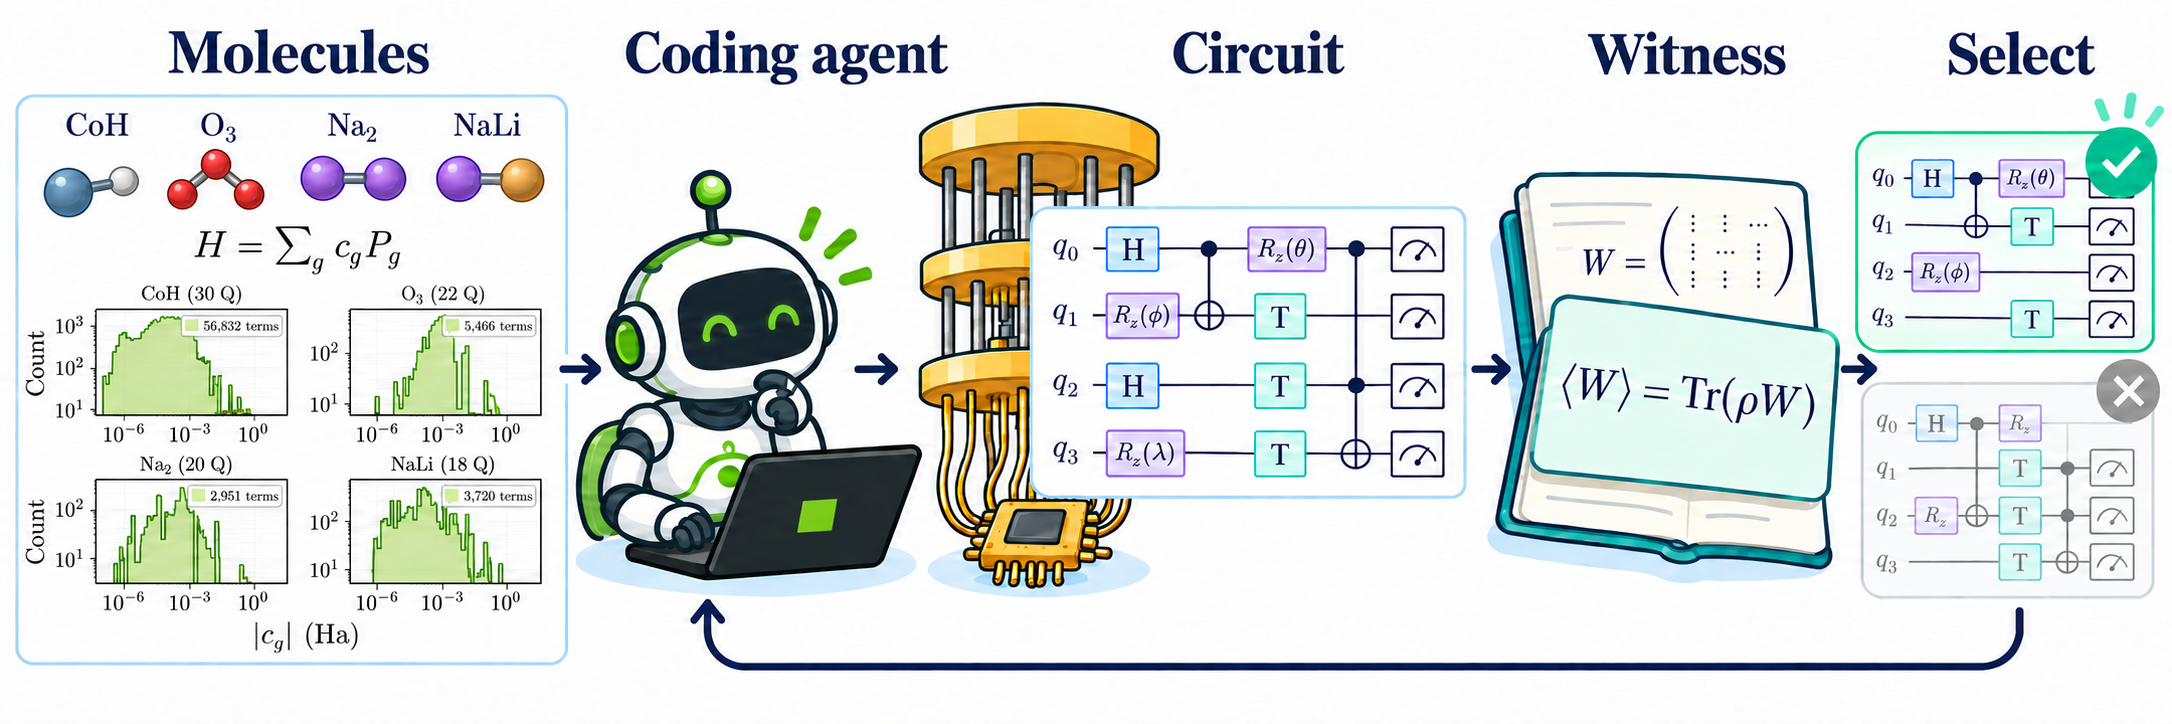
\includegraphics[width=2172pt,height=724pt]{generated-banner.png}};
\end{scope}
\end{pgfinterruptboundingbox}
% Circuit typography enlarged without enlarging the five section headings.
\foreach \y/\q in {380/0,310/1,240/2,150/{n-1}}{
 \node[anchor=east,font=\fontsize{27}{31}\selectfont] at (711,\y) {$q_{\q}$};
 \draw[line width=1.35pt] (721,\y)--(863,\y);
 \draw[line width=1.35pt] (900,\y)--(968,\y);
 \node[font=\fontsize{29}{32}\selectfont] at (881,\y) {$\cdots$};
}
\gate{746}{380}{H}\gate{746}{310}{T}\gate{746}{240}{H}\gate{746}{150}{H}
\cx{789}{380}{310}
\gate{820}{380}{T}\gate{820}{310}{T^\dagger}\gate{820}{240}{T}\gate{820}{150}{T}
\cx{856}{310}{240}
\gate{937}{380}{H}\gate{937}{310}{S}\gate{937}{240}{H}\gate{937}{150}{H}
\foreach \x in {698,829,937}{\node at (\x,195) {$\vdots$};}
\node at (835,100) {$U_{\mathcal P}(t)$};
% Error label is horizontal, above the plot, rather than rotated.
\node[font=\fontsize{30}{34}\selectfont] at (1120,403) {$|E_{\mathcal P}-E_0|$};
\fill[palegreen] (1038,150) rectangle (1220,280);
\draw[-{Latex[length=9pt,width=7pt]},line width=2pt] (1038,150)--(1038,365);
\draw[line width=1.5pt] (1038,150)--(1220,150);
\draw[green,dashed,line width=1.7pt] (1038,280)--(1220,280);
\node[anchor=south west,text=green,font=\fontsize{30}{34}\selectfont] at (1045,288) {$\varepsilon_{\rm chem}$};
\node[anchor=east,font=\fontsize{27}{31}\selectfont] at (1027,150) {$0$};
\draw[green,line width=1.1pt,densely dotted] (1095,150)--(1095,220);
\draw[muted,line width=1.1pt,densely dotted] (1175,150)--(1175,335);
\fill[green] (1095,220) circle (7pt);
\draw[muted,line width=3pt,line cap=round] (1168,328)--(1182,342) (1168,342)--(1182,328);
\node[text=green] at (1095,124) {$\mathcal P_a$};
\node[text=muted] at (1175,124) {$\mathcal P_b$};
% Shorter lines leave room for larger monospaced text.
\draw[green,fill=palegreen,line width=1.3pt,rounded corners=4pt] (1280,260) rectangle (1515,420);
\node[anchor=west,text=green,font=\fontsize{30}{34}\selectfont] at (1292,395) {$\mathcal P_a$};
\draw[green,line width=3.5pt,line cap=round,line join=round] (1474,395)--(1483,386)--(1500,404);
\node[anchor=west,font=\fontsize{26}{30}\selectfont\ttfamily] at (1292,358) {def PF(H):};
\node[anchor=west,font=\fontsize{26}{30}\selectfont\ttfamily] at (1305,325) {split\_a(H,dt)};
\node[anchor=west,font=\fontsize{26}{30}\selectfont\ttfamily] at (1305,292) {eps=f(c,w)};
\draw[linegray,fill=gategray,line width=1.3pt,rounded corners=4pt] (1280,78) rectangle (1515,238);
\node[anchor=west,text=muted,font=\fontsize{30}{34}\selectfont] at (1292,213) {$\mathcal P_b$};
\draw[muted,line width=3pt,line cap=round] (1478,206)--(1492,220) (1478,220)--(1492,206);
\node[anchor=west,text=muted,font=\fontsize{26}{30}\selectfont\ttfamily] at (1292,176) {def PF(H):};
\node[anchor=west,text=muted,font=\fontsize{26}{30}\selectfont\ttfamily] at (1305,143) {split\_b(H,dt)};
\node[anchor=west,text=muted,font=\fontsize{26}{30}\selectfont\ttfamily] at (1305,110) {eps=g(c,w)};
\foreach \a/\b in {383/411,641/677,975/1005,1241/1270}{\draw[-{Latex[length=15pt,width=12pt]},line width=4.5pt,preaction={draw=white,line width=10pt}] (\a,250)--(\b,250);}
\draw[-{Latex[length=15pt,width=12pt]},green,line width=4.5pt,rounded corners=12pt] (1405,65)--(1405,24)--(520,24)--(520,108);
\node[fill=white,inner xsep=14pt,text=green,font=\fontsize{28}{32}\selectfont] at (930,24) {Autoresearch};
\end{tikzpicture}
\end{document}
